\documentclass[14pt,titlepage]{extbook}
\usepackage[most]{tcolorbox}  
\newtcbox{\mymath}[1][]{%
    nobeforeafter, math upper, tcbox raise base,
    enhanced, colframe=magenta!30!magenta,
    colback=white!30, boxrule=2pt,
#1}

\usepackage[latin1]{inputenc}
\usepackage[T1]{fontenc}
\usepackage[portuges]{babel}

\usepackage{amsmath,amsthm,amssymb}
\usepackage{mathtools,empheq}
\usepackage{verbatim,url}
\usepackage{epsfig}
\usepackage[bf]{subfigure}
\usepackage[bf]{caption}
\usepackage{blkarray,multirow}

\usepackage{macrosfabbri,macrosfmoura}
\usepackage{url}
\usepackage{hyperref}
\hypersetup{%
%  colorlinks=false,
%  citecolor=black,
   pagebackref=true,
   breaklinks=true,
   colorlinks,
   linktoc=all
}%

%\usepackage[numbers]{natbib}
\usepackage{natbib}

% for quotes at beginning of chapters etc
\usepackage{epigraph}

% For setmarginsrb:
\usepackage{vmargin}

\usepackage{nomencl}
\usepackage{fancyhdr}
\setlength{\headheight}{15.2pt}

% commutative diags
\usepackage{tikz-cd}

% customize lists
\usepackage{enumitem}

\usepackage{algorithm, algorithmic}


\renewcommand{\cite}{\citep}
%\newcommand{\mynewpage}{{\mbox{BLANK PAGE}}\cleardoublepage}
%\newcommand{\mynewpage}{{\mbox{}}\cleardoublepage}
\newcommand{\mynewpage}{}
% For onehalfspacing or doublespacing:
%\usepackage{setspace}

%%%%%%%%%%%%%%%%%%%%%%%%%%%%%%%%%%%%%%%%%%%%%%%%%%%%%%%%%%%%%%%%%%%%%%%%%%%%%%%

\includeonly{%
  front-matter,
  intro,
  coordenadas,
  matrizes-transf,
  matrizes-rigid,
  homogeneas,
  axb,
  svd,
  qr,
  qr-householder,
  cholesky,
  scilab,
  antisimetricas-exp,
%  condicionamento,
  todo,
  refs,
}

\renewcommand{\nomname}{Table of Notations}
\makenomenclature

% -- Possible lems.sty
% TODO - include new command for epheq/aligned eqn environments with braces
\renewcommand{\qedsymbol}{$\blacksquare$}
%%%%%%%%%%%%%%%%%%%%%%%%%%%%%%%%%%%%%%%%
% You have two versions of the macro
% \draftnote{My note}. The first version puts notes (e.g. My note in the example)
% into the margin of your document. The second formats the note as nothing. You
% 'comment out' the version of the macro you don't want (using a % at the
% beginning of the line).
\newcommand{\draftnote}[1]{\marginpar{\tiny\raggedright\textsf{\hspace{0pt}#1}}}
%\newcommand{\draftnote}[1]{}
%
% This one is just for the comments for in-line text.
\newcommand{\indraftnote}[1]{\textcolor{blue}{\texttt{\footnotesize [#1]}}}
\newcommand{\todo}[1]{\indraftnote{todo: #1}} % Este  "a fazer" � para eu n�o esquecer

\def\FigureFont{\footnotesize}
\def\TableFont{\small}
\def\SectionTitleFont{\large}
\def\TextFont{\normalsize}
\def\ReferenceFont{\normalsize}
\def\Reducefigspace{\vspace{-0.7 truecm}} %0.3
\def\ReduceRDfigspace{\vspace{-1.51truecm}}
\def\ReduceEndFigSpace{\vspace{-0.01 truecm}} %0.38
\def\ReduceRefSpace{\vspace{-0.01 truecm}} %0.5
\def\SectionSpacing{\vspace{0.5 truecm}} %0.25
\def\SubSectionSpacing{\vspace{0.5 truecm}} %0.25
\def\subsubsection#1{\par\medskip\noindent{\bf #1}\quad\nopagebreak}
\def\Bibspace{\vspace{-0.5cm}}
\def\ReduceSubsectionBelow{\vspace{-0.2cm}}
\def\ReduceSubsectionAbove{\vspace{-0.5cm}}
\def\IncreaseSubSubSectionAbove{\vspace{0.2cm}}
\def\ReduceEqSpace{\vspace{-0.1cm}}
\def\ReduceSecSpace{\vspace{-0.1cm}}


\newcommand{\intinf}{\int_{-\infty}^{\infty}}
\newcommand{\grad}{\nabla}
\newcommand{\slant}{\sigma}
\newcommand{\R}{\mathbb{R}} % the reals
\newcommand{\trace}{\text{trace}\,}
%\newcommand{\det}{\text{det}}

% skew-symmetric arrangement
\newcommand{\skewm}[1]{{#1}_\times}

\renewcommand{\vec}[1]{\mathbf{#1}}

\newcommand{\lbar}{\overline}

\newcommand{\id}{\text{\emph{I}}}
\newcommand{\dof}{\textsc{dof}}
\newcommand{\ransac}{\textsc{ransac}}
\newcommand{\sift}{\textsc{sift}}
\newcommand{\klt}{\textsc{klt}}
\newcommand{\svd}{\textsc{svd}}
\newcommand{\sfm}{\textsc{sfm}}
\newcommand{\rot}{\mathcal{R}}
\newcommand{\brot}{\overline{\mathcal{R}}}

\def\bsq#1{%both single quotes
\lq{#1}\rq}

% The following are not very good constructs it seems. Better to use just
% \begin{bmatrix}..\end{\bmatrix}

\newcommand{\datsqbr}[2][rrrrrrrrrrrrrrrrrrrrrrrrrrrrrrrrrrrr]{\left[
\begin{array}{#1}
#2\\
\end{array}
\right]
}


% -- !lems.sty

%%%%%%%%%%%%%%%%%%%%%%%%%%%%%%%%%%%%%%%%%%%%%%%%%%%%%%%%%%%%%%%%%%%%%%%%%%%%%%%
%\setmarginsrb{30mm}{27mm}{20mm}{20mm}{12pt}{25pt}{0pt}{5mm}
\setmarginsrb{20mm}{27mm}{20mm}{25mm}{12pt}{25pt}{0pt}{10mm}
%             left   top  right bottom headheight headsep footheight footsep 


\newtheorem{thm}{Theorem}
\newtheorem{lem}[thm]{Lemma}

\newtheorem{theorem}{Theorem}[section]
\newtheorem{corollary}[theorem]{Corollary}
\newtheorem{corolary}[theorem]{Corollary}
\newtheorem{proposition}[theorem]{Proposition}
\newtheorem{lemma}[theorem]{Lemma}

\theoremstyle{definition}
\newtheorem{definition}{Definition}
\newtheorem{remark}{Remark}[section]
\newtheorem{problem}{Problem}[section]
\newtheorem{question}{Question}[section]
\newtheorem{property}{Property}
\newtheorem{example}{Example}
\newtheorem{transformation}{Transformation}

\numberwithin{equation}{chapter}

\newcommand{\Gama}{\boldsymbol{\Gamma}}
\newcommand{\gama}{\boldsymbol{\gamma}}
\newcommand{\gamad}{\dot{\gama}}
\newcommand{\bsigma}{\boldsymbol{\sigma}}
\newcommand{\T}{\boldsymbol{T}}
\newcommand{\N}{\mathbf{N}}
\newcommand{\NSurface}{\mathbf{N}}
\newcommand{\Nlocal}{\overline{\N}} % normal in local coordinates
\newcommand{\balpha}{\boldsymbol{\alpha}}
\newcommand{\tDt}{t+\Delta t}
\newcommand{\bpsi}{\boldsymbol{\boldsymbol{\psi}}}
\newcommand{\bp}{\mathbf p}
\newcommand{\deldt}[1]{\frac{\partial#1}{\partial t}}
\newcommand{\ddt}[1]{\frac{d #1}{dt}}
\newcommand{\delds}[1]{\frac{\partial#1}{\partial s}}
\newcommand{\mybar}[1]{\overline{#1}}
\newcommand{\norm}[1]{\|#1\|}
\newcommand{\I}{\mathbf{I}}
\newcommand{\brho}{\boldsymbol{\rho}}
\newcommand{\lightrgb}{\boldsymbol{l}}
\newcommand{\B}{\boldsymbol{B}}
\renewcommand{\t}{\boldsymbol{t}}
\newcommand{\n}{\boldsymbol{n}}
\renewcommand{\b}{\boldsymbol{b}}
\newcommand{\e}{\boldsymbol{e}}
\newcommand{\f}{\boldsymbol{F}}
\newcommand{\hf}{\boldsymbol{\hat{f}}}
\newcommand{\g}{\boldsymbol{g}}
\newcommand{\G}{\boldsymbol{G}}
\newcommand{\bc}{\boldsymbol{c}}
\newcommand{\Curve}{\boldsymbol{\mathcal{C}}}
%\newcommand{\X}{\boldsymbol{X}}
%\newcommand{\x}{\boldsymbol{x}}
\newcommand{\X}{\mathbf{X}}
\newcommand{\x}{\mathbf{x}}
\newcommand{\xx}{\mathcal{X}}  % used in Giblin's notes
\newcommand{\tilx}{\tilde x}
\newcommand{\tily}{\tilde y}
\newcommand{\tilgama}{\tilde \gama}
\newcommand{\ugama}{\hat{\gama}} %unit gama
\newcommand{\br}{\bar r}
\newcommand{\Kc}{\mathbf K_c}
\newcommand{\lepi}{\mathbf r}
\newcommand{\itan}{\tan^{-1}}
\newcommand{\uu}{\xi}
\newcommand{\buu}{\bar \uu}
\newcommand{\bvv}{\bar \vv}
\newcommand{\vv}{\eta}
\newcommand{\VV}{\mathbf{V}} % translational velocity
\newcommand{\VVspeed}{V} % translational velocity
\newcommand{\field}{\boldsymbol\chi}
\newcommand{\ufield}{\hat{\boldsymbol{\chi}}}
\newcommand{\fieldc}{\chi} % field component
\newcommand{\transl}{\mathcal{T}} % field component
\newcommand{\btransl}{\overline{\mathcal{T}}} % field component
\newcommand{\albedo}{\alpha}
\newcommand{\depth}{\rho}      % depth as z
\newcommand{\ddepth}{\dot{\rho}}      % depth as z
\renewcommand{\l}{\lambda} % used in problem2-thoughts-giblin
\newcommand{\udepth}{{\hat{\rho}}} % depth along ray
\newcommand{\ttransl}{\T} % translation tangent
\newcommand{\surface}{\mathcal{M}} % surface/manifold
\newcommand{\surf}{\mathcal{M}} % surface/manifold short
\newcommand{\jacm}{\mathtt{J}} % Jacobian matrix
\newcommand{\xbar}{\bar x}
\newcommand{\ybar}{\bar y}
\newcommand{\zbar}{\bar z}

\newcommand{\bdelta}{\boldsymbol \delta}
%\newcommand{\X}{\boldsymbol{X}}
%\newcommand{\x}{\boldsymbol{x}}
%\newcommand{\X}{\mathbf{X}}
%\newcommand{\x}{\mathbf{x}}
\newcommand{\boldu}{\mathbf{u}}
\newcommand{\boldv}{\mathbf{v}}
\newcommand{\boldw}{\mathbf{w}}
\newcommand{\tgtveloc}{\tilde\alpha} % real tangential velocity

\makeindex
\setcounter{tocdepth}{1}

\addto\captionsenglish{\renewcommand{\chaptername}{Lecture}}
\addto\captionsportuges{\renewcommand{\chaptername}{Aula}}

\begin{document}

%\authorrunning{Fabbri and Kimia}
%\mynewpage
%\listoffigures
%\onehalfspacing
\begin{titlepage}
\begin{center}

 % \vspace*{0.4cm}

 % \includegraphics[width=2.5cm, height=2.5cm]{v1.png}

\includegraphics[height=1.5cm]{figs/iprj-heading-v1.png}
  \vspace{2cm}

%\begin{minipage}[b]{12cm}\noindent
%    \begin{center}
%      {\Large Universidade do Estado do Rio de Janeiro} \\ {\Large
%	Instituto Politécnico - \Large IPRJ}
%    \end{center}
%  \end{minipage}

 % \Large

  %\sffamily

  %\vspace{0.4cm}

\begin{center}
 % {\LARGE \textbf{Método de redução de dimensionalidade não linear: um estudo sobre aplicação de difusão}}
% {\huge \textbf {Um estudo de redução de\vskip1cm
 %  dimensionalidade  por difusão}} \vskip1cm
  {\huge \textbf {Álgebra Linear Numérica }}
  \vskip1cm 
 
\end{center}

  \vspace{0.6cm}
  {\LARGE \textbf{Notas de Aula}}

\vspace{10 cm} % eu coloquei este que não tinha

\begin{center}
\textbf{Ricardo Fabbri}
\end{center}


 \begin{center}
  \vspace{0.5 cm}
 
% \usdate
 {\large \textbf{\today}}%\currenttime}}
\end{center}
\end{center}
\end{titlepage}
\thispagestyle{empty}
\frontmatter

\tableofcontents
%\listoffigures
%\printnomenclature[3.5cm]
\mainmatter
\pagestyle{fancy}
\fancyhead[LE]{\nouppercase{\leftmark}}
\fancyhead[RE]{\thepage}
\fancyhead[LO]{\nouppercase{\rightmark}}
\fancyhead[RO]{\thepage}
\mynewpage
\chapter{O que � uma matriz?}

\section*{Objetivos}
\begin{itemize}
\item Aula introdut�ria informal dando vis�o geral e uma contextualiza��o do curso
\item Motivar alunos de engenharia da computa��o da import�ncia da disciplina ao
  final do curso, no contexto de modelagem computacional do IPRJ/UERJ.
\item O que � �lgebra linear num�rica: explicar termos ``�lgebra'', ``linear'',
  e ``num�rica''. Por qu� s�o importantes.
\item Matrizes como representa��o num�rica de transforma��es lineares
\item Crit�rio de avalia��o
\end{itemize}

\subsection*{O que � uma matriz?}
\begin{itemize}
\item Uma tabela retangular de n�meros, por�m n�o s�. 
\item Associados � tabela h� uma ``�lgebra'': opera��es alg�bricas
  usuais de multiplica��o matriz-vetor e matriz-matriz vistas no ensino m�dio,
  que parecem arbitr�rias.
\item Quando falamos de matrizes em engenharia e ci�ncia, sempre incluimos, portanto, tais opera��es.
\item O curso se chama �lgebra Linear Num�rica. At� agora, ent�o, falamos algo
  de ``num�rico'' (matrizes s�o um monte de n�meros) e de ``alg�bra''
  (opera��es). E o ``linear''?
\item Matrizes s�o representa��es num�ricas de transforma��es lineares.
\end{itemize}

\subsection*{O que � ``Linear''?}
\begin{itemize}
\item Ao ouvir a palavra ``linear'', a maioria das pessoas tem em mente uma reta ou um
plano.
\item ``Linearidade'' em matem�tica � uma forma de ``simplicidade''.
\item Esta simplicidade se manifesta em diversos n�veis: o geom�trico, o
  simb�lico, e o num�rico:
\end{itemize}
   
\paragraph{Simb�lico:}
No plano simb�lico ou alg�brico, explica-se os fen�menos de forma operacional e
abstrata, sem muita intui��o conceitual sobre o significado dos s�mbolos ou opera��es.
\begin{defi} \emph{(Simbolicamente Linear)} \label{def:linear:symbolic}
Muitos matem�ticos ir�o definir ``linear'' como a
  qualidade de uma fun��o ou transforma��o $L$ tal que 
  \begin{empheq}[left=\empheqlbrace]{align}
    &L(v + w) = L(v) + L(w)\\
    &L(\alpha v) = \alpha L(v),
    \label{eq:linear:symbolic}
  \end{empheq}
  para todos vetores $v$ e $w$, e escalares $\alpha$.
\end{defi}
\begin{itemize}
\item Tal defini��o, apesar de suscinta e formalmente elegante, tem pouca
  concretude imediata.
\item ``Linear'' aqui significa apenas uma simplicidade formal, ou seja, as
  manipula��es alg�bricas s�o simples.
\end{itemize}

\paragraph{Geom�trico:} No plano que aqui chamamos de ``geom�trico'',
``conceitual'', ou ``visual'', os fen�menos s�o explicados de maneira concreta,
mais pr�xima do objetivo ou de aplica��es reais. 

No mundo real, o que observamos
a princ�pio n�o � num�rico nem simb�lico: uma bola girando, um fl�ido em movimento, ou um feixe de n�utrons.
Muitas vezes, conceitos pr�ximos da realidade, independentes das conven��es de s�mbolos ou
n�meros, s�o dif�ceis de formalizar e, portanto, n�o s�o enfatizados na maioria
dos cursos de �lgebra linear.
\begin{defi} \emph{(Geometricamente Linear)}
  Chama-se ``Linear'' qualquer opera��o geom�trica que combina quaisquer das seguintes
  opera��es simples: girar, esticar e refletir.
  \label{def:linear:geometric}
\end{defi}

\begin{itemize}
\item Tais opera��es s�o globais e realizadas sobre um mesmo ponto central (origem)
\item O esticamento pode ser realizado por fatores diferentes ao longo de eixos arbitr�rios, e inclui achatamentos
\item Geralmente, esta defini��o � um teorema na teoria da �lgebra linear, visto
  apenas no final de um primeiro curso.  Trata-se
  do teorema do SVD -- \emph{Singular Value Decompositon}, ou decomposi��o em
  valores singulares. Trata-se de um an�logo de autovalores e autovetores, e � o
  teorema mais importante a ser explorado neste curso.
\item Como exemplo, temos a seguinte figura:
  \begin{center}
  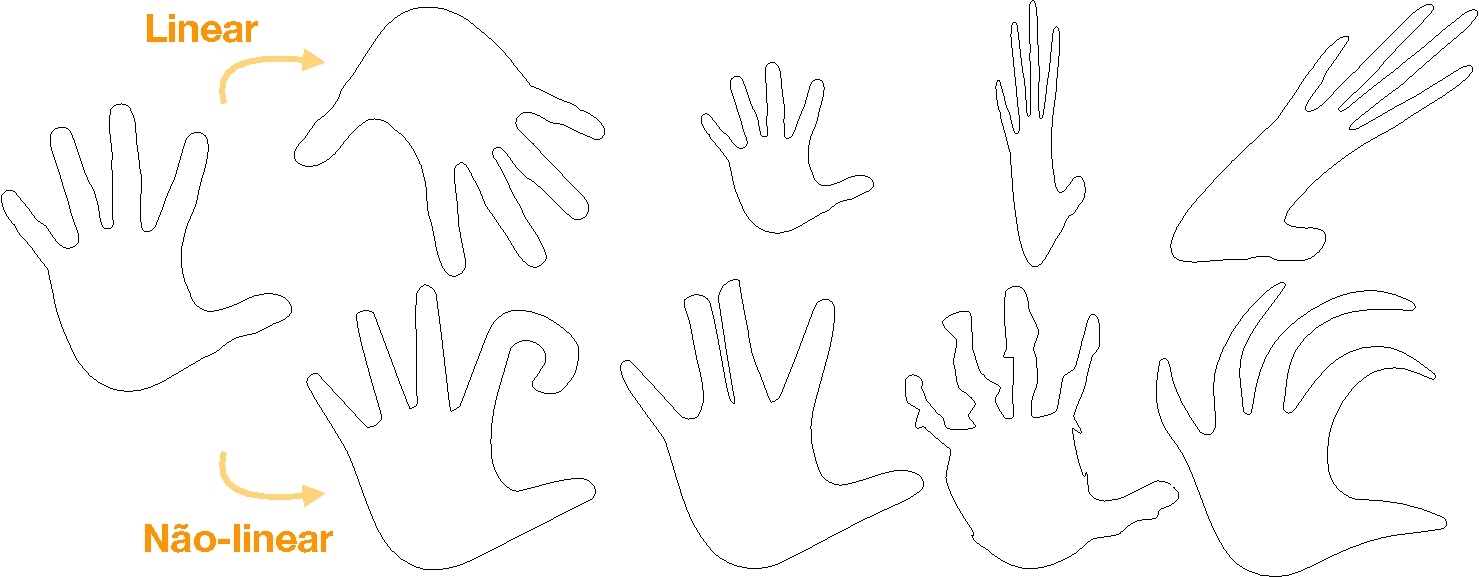
\includegraphics[scale=0.5]{figs/nonlinear-transf-hands.pdf}
  \end{center}
  A m�o � esquerda sofre transforma��es lineares na linha acima, e n�o-lineares
  na linha abaixo. As transforma��es acima s�o lineares pois consistem em
  girar ou esticar cada ponto da m�o globalmente pelo mesmo �ngulo ou fatores de
  esticamento. J� as transforma��es na linha abaixo s�o n�o-lineares pois os
  pontos ou sofrem deforma��es locais (diferentes para cada ponto da m�o), ou
  n�o s�o meramente girados e esticados.
\end{itemize}

\paragraph{Num�rico:} J� definimos no in�cio da aula que uma matriz � a
representa��o num�rica de uma transforma��o linear, seja esta pensada pela
defini��o geom�trica ou simb�lica. 
\begin{itemize}
\item Para maior compreens�o do significado dos n�meros e opera��es de uma
  matriz, na pr�xima aula revisaremos o conceito de \emph{coordenadas}.
\item Tamb�m revisaremos como encontrar os n�meros em uma matriz para uma dada
  transforma��o linear
\end{itemize}
O teorema do SVD pode ser descrito num�ricamente em termos de matrizes:
\begin{teo}\label{teo:svd:informal}
  (SVD numerico - informal)
  Toda matriz A de tamanho $m\times n$ pode ser escrita da forma:
  \begin{center}
  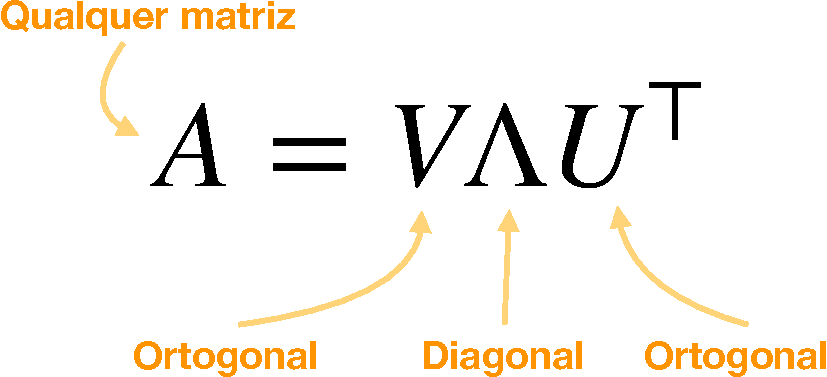
\includegraphics[scale=0.5]{figs/svd-matricial.pdf}
  \end{center}
  Ou seja, toda matriz � uma matriz diagonal junto com matrizes ortogonais.
  A matriz diagonal realiza esticamento em cada eixo, e as matrizes ortogonais
  realizam rota��es e reflex�es. 
\end{teo}
\begin{itemize}
\item O tamanho das matrizes �
  \begin{equation}
   A_{m\times n} = V_{m\times m}\,\Lambda_{m\times n}\, U_{n \times n}^\top 
  \end{equation}
\item Portanto toda matriz �, de certa forma, equivalente a uma matriz diagonal de mesmo
  tamanho.
\item Matrizes diagonais s�o matrizes da seguinte forma (exemplo $3\times 3$):
  \begin{equation}
    \Lambda = 
    \begin{bmatrix}
     a & 0 & 0 \\
     0 & b & 0 \\
     0 & 0 & c \\
   \end{bmatrix},
    \label{eq:diagonal}
  \end{equation}
  as quais transformam pontos $(x,y,z)$ da seguinte forma:
  \begin{equation}
    \Lambda = 
    \begin{bmatrix}
     a & 0 & 0 \\
     0 & b & 0 \\
     0 & 0 & c \\
    \end{bmatrix}
    \begin{bmatrix}
      x\\
      y\\
      z
    \end{bmatrix}
    = 
    \begin{bmatrix}
      a x\\
      b y\\
      c z
    \end{bmatrix},
  \end{equation}
  ou seja, esticam cada ponto ao longo de eixos por fatores $a$, $b$ e $c$. 
\item Cada fator de esticamento $a$, $b$ ou $c$ pode ser zero, o que faz com que
  a matriz achate completamente uma das dimens�es
\end{itemize}

\paragraph{Observa��es}
\begin{itemize}
\item A transla��o � n�o-linear. Pode-se mostrar que, mesmo sendo uma opera��o
  geom�trica simples, a transla��o n�o tem as propriedades de simplicidade
  alg�brica como na defini�ao simb�lica acima, e tamb�m n�o pode ser expressa
  numericamente como uma multiplica��o de matrizes. 
\item Com alguns artif�cios, � poss�vel realizar transla��o com multiplica��o de matrizes,
  por�m � preciso opera��es n�o-lineares (proje��o).
\end{itemize}

\paragraph{Para qu� servem as transforma��es lineares, se elas s�o t�o
limitadas?}

\begin{itemize}
\item O mundo real � n�o-linear
\item O ``Linear'' foi inventado como uma simplifica��o do n�o-linear, mas em si
  n�o tem aplica��o pr�tica.
\item O linear n�o faz sentido sem o n�o-linear. 
\item O linear s� existe como artefato para modelar o n�o-linear.
\item O paradigma � tomar um fen�meno real (e n�o-linear) e lineariz�-lo, para
  usar as ferramentas deste curso.
\item Em C�lculo 1, estudamos fun��es n�o-lineares de uma vari�vel usando
  a derivada como lineariza��o local (reta tangente). A reta tangente � uma
  transforma��o linear de uma vari�vel.
\item Da� a import�ncia de se estudar cursos como an�lise no $\mathbb R^n$, onde
  fen�menos n�o-lineares s�o modelados tendo como
  ferramenta b�sica a �lgebra linear.
\item �lgebra linear tamb�m � o primeiro contato do aluno com $n$ dimens�es,
  para $n > 3$, e tem import�ncia direta na pr�tica, por exemplo em intelig�ncia artificial,
\emph{machine learning}.
\item Por exemplo, o paradigma de c�lculo e an�lise no $\mathbb R^n$ � estudar o
  n�o-linear realizando lineariza��es locais (diferencia��o). Dessa forma, para
  se deformar a m�o de forma mais geral, como na figura abaixo, pode-se usar
  v�rias transforma��es lineares com fatores de esticamento e rota��o diferentes para cada ponto:
  \begin{center}
  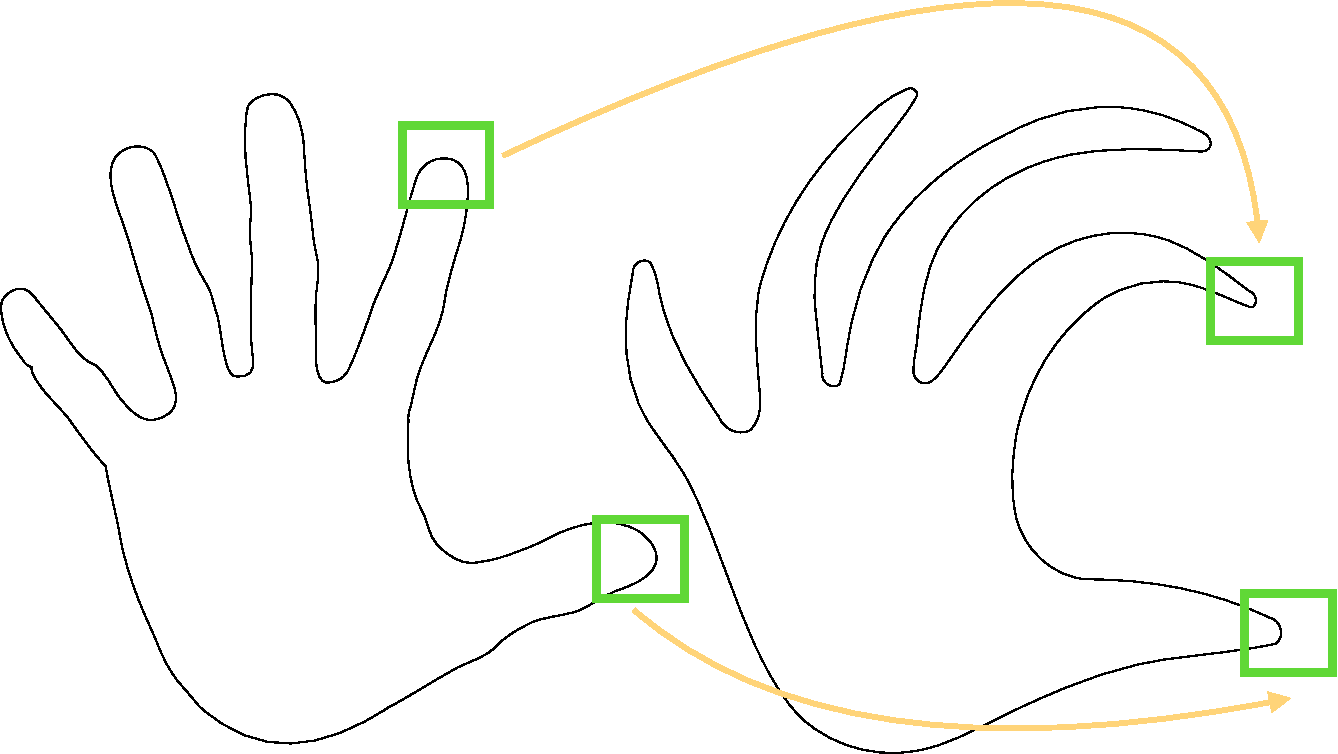
\includegraphics[scale=0.5]{figs/nonlinear-using-linear.pdf}
  \end{center}
\item Em cada quadrado verde, temos uma deforma��o pr�xima de uma rota��o e um
  esticamento.
\item Curiosidade: a deforma��o n�o-linear da m�o � uma fun��o de $\mathbb R^2
  \to \mathbb R^2$ estudada em An�lise no $\mathbb R^n$. A aproxima��o da
  deforma��o de cada quadrado verde � chamada de diferencial da fun��o
  n�o-linear, e sua forma num�rica (matricial) � estudada em �lgebra linear
  num�rica.
\end{itemize}

\subsection*{Tarefas}

\begin{itemize}
\item Site: \url{http://wiki.nosdigitais.teia.org.br/ALN}
\item Realizar tarefa 0 e tarefa 1 (datas no site).
\end{itemize}

\subsection*{Exerc�cios}
\begin{enumerate}
\item Explique como uma fun��o $f: \mathbb R \to \mathbb R$, $y = f(x)$, seria
  considerada linear, tanto em termos s�mb�licos e geom�tricos. Qual seria a
  f�rmula dessa fun��o?
\end{enumerate}

\mynewpage
\chapter{Revis�o de �lgebra Linear}

\section*{Objetivos}
\begin{itemize}
\item Relebrar representa��o num�rica de transforma��es lineares
\item Revisar �lgebra linear n�o-num�rica (``simb�lica'')
\item Estilo: revis�o aprofundada para alunos que ja viram a disciplina. Nota��o
solta adequada a uma revis�o.
\end{itemize}

\section*{Observa��es Iniciais}
\begin{itemize}
\item A �lgebra liner num�rica come�a com o conceito de escalares e coordenadas.
\item Para haver coordenadas, � necess�ria a escolha da escolha de uma base
\item O conceito de espa�o vetorial (simb�lico) permite isolar as opera��es
  que n�o dependem da escolha de uma base, daquelas que dependem.
\end{itemize}

\begin{defi} \emph{(Espa�o Vetorial Simb�lico)}
Um espa�o vetorial $\mathcal V$ sobre um corpo $K$ � uma tupla ordenada
$\mathcal V = (V, K, +, \cdot)$ de quatro elementos:
\begin{empheq}[left=\mathcal V\ \ \empheqlbrace]{align}
  &V\text{: conjunto cujos elementos s�o chamados ``vetores''}\nonumber\\
  &K\text{: conjunto cujos elementos s�o chamados ``escalares''}\nonumber\\
  &+\text{: soma de vetores}\nonumber\\
  &\cdot\text{: multiplica��o vetor-escalar,}\nonumber
\end{empheq}
onde ``+'' satisfaz:
\begin{align}
  +: V \times V &\to V\\
  (v,w) &\mapsto v+w,
\end{align}
\begin{align}
  &v + w = w + v\\
  &v + (u + w) = (v + u) + w\\
  &\exists !\ 0 \in V \text{ tal que } 0 + v = v,\ \forall v\in V\\
  &\forall v \in V, \exists !\ w \in V \text{ tal que } v + w = 0, \text{simbolizado por } -v
\end{align}
e onde ``$\cdot$'' satisfaz:
\begin{align}
  \cdot: K \times V &\to V\\
  (\alpha,w) &\mapsto v+w,
\end{align}
\begin{align}
  &v + w = w + v\\
  &v + (u + w) = (v + u) + w\\
  &\exists !\ 0 \in V \text{ tal que } 0 + v = v,\ \forall v\in V\\
  &\forall v \in V, \exists !\ w \in V \text{ tal que } v + w = 0, \text{simbolizado por } -v
\end{align}
e $K$ satisfaz as propriedades de uma estrutura alg�bridca chamada ``corpo'',
que abstrai as opera��es de multiplica��o, soma, subtra��o e divis�o poss�veis
com n�meros, geralmente $\mathbb R$ ou $\mathbb C$.
\end{defi}

\begin{itemize}
\item Aos programadores em C++: a defini��o de espa�o vetorial simb�lico � como uma
  \emph{classe}, que define as partes e as opera��es permitidas. 
\item Na defini��o simb�lica um vetor � apenas caracterizado pelas opera��es que
  se pode realizar com ele, e as propriedades de tais opera��es.
\item At� o momento, a �nica coisa ``num�rica'' nesta defini��o � o  
  corpo de escalares $K$. Os vetores ainda s�o entidades simb�licas que podem ser somadas e
  multiplicadas por escalar.
\item A teoria simb�lica parece artificialmente trivial -- todos j� sabemos as
  propriedades convencionais de soma de vetores e multiplica��o por
  escalar. 
\item No entanto, a teoria simb�lica est� mais pr�xima do conceitual que a
  teoria num�rica, pois isola os fatores que n�o dependem da escolha de um
  sistema de coordenada.
\item A conex�o com o mundo num�rico consiste em associar n�meros a vetores.
  Para tanto, � importante definir base e, para isso, depend�ncia linear.
\item Iremos assumir que $V$ e $W$ s�o espa�os vetoriais.
\end{itemize}

\begin{defi}
  Uma combina��o linear de $v_1,\dots,v_n$, $v_i \in V$, � uma express�o da
  forma
  \begin{equation}
    \alpha_1 v_1 + \dots + \alpha_n v_n = \sum \alpha_i v_i.
  \end{equation}
\end{defi}
\begin{itemize}
\item Nota��o: quando n�o h� ambuguidade, iremos omitir os �ndices dos
  somat�rios $\sum$.
\end{itemize}
\begin{defi}
  Os vetores $v_1,\dots,v_n$ s�o ditos linearmente indepententes (L.I.) se
  \begin{equation}
    \sum \alpha_i v_i\ \  \iff\ \  \alpha_i = 0\,\ i=1,\dots,n
  \end{equation}
\end{defi}

\begin{prop}
  $v_1,\dots,v_n$ s�o L.I. se, e somente se, cada $v_i$ n�o � o vetor nulo (isto
    �, $v_i \neq 0$) e nenhum � combina��o linear dos demais 
\end{prop}

\begin{defi}
  $\{v_1,\dots,v_n\} \subset V$ � base de $V$ se
\begin{empheq}[left=\empheqlbrace]{align}
  &v_1,\dots,v_n \text{ s�o L.I. e}\\
  &\text{todo $v \in V$ � combina��o linear dos $v_i$'s}
\end{empheq}
\end{defi}

Finalmente, chegamos ao conceito de coordenadas (num�ricas) de um vetor:
\begin{defi} \emph{(Coordenadas)} Dada uma base $B = \{v_1,\dots,v_n\}$ de $V$,
ent�o os n�meros $\alpha_1,\dots,\alpha_n$ tal que
  \begin{equation}
    v = \sum \alpha_i v_i
  \end{equation}
  s�o chamados de coordenadas de $v$ em $V$ (na base $B$). Quando necess�rio,
  utiliza-se a nota��o expl�cita: 
  \begin{equation}
  \mathcal X_B(v) = 
  \begin{bmatrix}
    \alpha_1\\
    \alpha_n
  \end{bmatrix},
  \end{equation}
  onde o s�mbolo ``chi'' $\mathcal X$ dever ser lido como ``coordenada de''.
\end{defi}

\begin{itemize}
\item Se pensarmos no vetor simb�lico $v\in V$ visualmente como uma seta desenhada no plano, suas
coordenadas s�o um vetor num�rico $2$ n�meros, sendo necess�rio definir a base
(posi��o dos eixos $x$ e $y$).
\item Fixada uma base, existe uma rela��o 1-1 entre vetores simb�licos $v$ e
  vetores de $n$ n�meros.
\end{itemize}

\begin{teo}
  Dada uma base de $n$ vetores, tem-se que:
  \begin{itemize}
  \item As $n$ coordenadas de um vetor s�o �nicas
  \item Qualquer outra base de $V$ tem o mesmo n�mero de elementos $n$, que usaremos como
    a defini��o da dimens�o de $V$.
  \end{itemize}
\end{teo}
\dem
Ambos decorrem de propriedades de sistemas lineares. Os detalhes j� foram
vistos pelo aluno no primeiro curso de �lgebra linear.
\fim


\mynewpage
\chapter{Revis�o de �lgebra Linear}

\section*{Objetivos}
\begin{itemize}
\item Relebrar representa��o num�rica de vetores 
\item Revisar �lgebra linear n�o-num�rica (``simb�lica'')
\item Estilo: revis�o aprofundada para alunos que ja viram a disciplina. Nota��o
solta adequada a uma revis�o.
\end{itemize}

\section*{Observa��es Iniciais}
\begin{itemize}
\item A �lgebra liner num�rica come�a com o conceito de escalares e coordenadas.
\item Para haver coordenadas, � necess�ria a escolha da escolha de uma base
\item O conceito de espa�o vetorial (simb�lico) permite isolar as opera��es
  que n�o dependem da escolha de uma base, daquelas que dependem.
\end{itemize}

\begin{defi} \emph{(Espa�o Vetorial Simb�lico)}
Um espa�o vetorial $\mathcal V$ sobre um corpo $K$ � uma tupla ordenada
$\mathcal V = (V, K, +, \cdot)$ de quatro elementos:
\begin{empheq}[left=\mathcal V\ \ \empheqlbrace]{align}
  &V\text{: conjunto cujos elementos s�o chamados ``vetores''}\nonumber\\
  &K\text{: conjunto cujos elementos s�o chamados ``escalares''}\nonumber\\
  &+\text{: soma de vetores}\nonumber\\
  &\cdot\text{: multiplica��o vetor-escalar,}\nonumber
\end{empheq}
onde ``+'' satisfaz:
\begin{align}
  +: V \times V &\to V\\
  (v,w) &\mapsto v+w,
\end{align}
\begin{align}
  &v + w = w + v\\
  &v + (u + w) = (v + u) + w\\
  &\exists !\ 0 \in V \text{ tal que } 0 + v = v,\ \forall v\in V\\
  &\forall v \in V, \exists !\ w \in V \text{ tal que } v + w = 0, \text{simbolizado por } -v
\end{align}
e onde ``$\cdot$'' satisfaz:
\begin{align}
  \cdot: K \times V &\to V\\
  (\alpha,w) &\mapsto v+w,
\end{align}
\begin{align}
  &v + w = w + v\\
  &v + (u + w) = (v + u) + w\\
  &\exists !\ 0 \in V \text{ tal que } 0 + v = v,\ \forall v\in V\\
  &\forall v \in V, \exists !\ w \in V \text{ tal que } v + w = 0, \text{simbolizado por } -v
\end{align}
e $K$ satisfaz as propriedades de uma estrutura alg�bridca chamada ``corpo'',
que abstrai as opera��es de multiplica��o, soma, subtra��o e divis�o poss�veis
com n�meros, geralmente $\mathbb R$ ou $\mathbb C$.
\end{defi}

\begin{itemize}
\item Aos programadores em C++: a defini��o de espa�o vetorial simb�lico � como uma
  \emph{classe}, que define as partes e as opera��es permitidas. 
\item Na defini��o simb�lica um vetor � apenas caracterizado pelas opera��es que
  se pode realizar com ele, e as propriedades de tais opera��es.
\item At� o momento, a �nica coisa ``num�rica'' nesta defini��o � o  
  corpo de escalares $K$. Os vetores ainda s�o entidades simb�licas que podem ser somadas e
  multiplicadas por escalar.
\item A teoria simb�lica parece artificialmente trivial -- todos j� sabemos as
  propriedades convencionais de soma de vetores e multiplica��o por
  escalar. 
\item No entanto, a teoria simb�lica est� mais pr�xima do conceitual que a
  teoria num�rica, pois isola os fatores que n�o dependem da escolha de um
  sistema de coordenada.
\item A conex�o com o mundo num�rico consiste em associar n�meros a vetores.
  Para tanto, � importante definir base e, para isso, depend�ncia linear.
\item Iremos assumir que $V$ e $W$ s�o espa�os vetoriais.
\end{itemize}

\begin{defi}
  Uma combina��o linear de $v_1,\dots,v_n$, $v_i \in V$, � uma express�o da
  forma
  \begin{equation}
    \alpha_1 v_1 + \dots + \alpha_n v_n = \sum \alpha_i v_i.
  \end{equation}
\end{defi}
\begin{itemize}
\item Nota��o: quando n�o h� ambuguidade, iremos omitir os �ndices dos
  somat�rios $\sum$.
\end{itemize}
\begin{defi}
  Os vetores $v_1,\dots,v_n$ s�o ditos linearmente indepententes (L.I.) se
  \begin{equation}
    \sum \alpha_i v_i\ \  \iff\ \  \alpha_i = 0\,\ i=1,\dots,n
  \end{equation}
\end{defi}

\begin{prop}
  $v_1,\dots,v_n$ s�o L.I. se, e somente se, cada $v_i$ n�o � o vetor nulo (isto
    �, $v_i \neq 0$) e nenhum � combina��o linear dos demais 
\end{prop}

\begin{defi}
  $\{v_1,\dots,v_n\} \subset V$ � base de $V$ se
\begin{empheq}[left=\empheqlbrace]{align}
  &v_1,\dots,v_n \text{ s�o L.I. e}\\
  &\text{todo $v \in V$ � combina��o linear dos $v_i$'s}
\end{empheq}
\end{defi}

Finalmente, chegamos ao conceito de coordenadas (num�ricas) de um vetor:
\begin{defi} \emph{(Coordenadas)} Dada uma base $B = \{v_1,\dots,v_n\}$ de $V$,
ent�o os n�meros $\alpha_1,\dots,\alpha_n$ tal que
  \begin{equation}
    v = \sum \alpha_i v_i
  \end{equation}
  s�o chamados de coordenadas de $v$ em $V$ (na base $B$). Quando necess�rio,
  utiliza-se a nota��o expl�cita: 
  \begin{equation}
  \mathcal X_B(v) = 
  \begin{bmatrix}
    \alpha_1\\
    \alpha_n
  \end{bmatrix},
  \end{equation}
  onde o s�mbolo ``chi'' $\mathcal X$ dever ser lido como ``coordenada de''.
\end{defi}

\begin{itemize}
\item Se pensarmos no vetor simb�lico $v\in V$ visualmente como uma seta desenhada no plano, suas
coordenadas s�o um vetor num�rico $2$ n�meros, sendo necess�rio definir a base
(posi��o dos eixos $x$ e $y$).
\item Fixada uma base, existe uma rela��o 1-1 entre vetores simb�licos $v$ e
  vetores de $n$ n�meros.
\end{itemize}

\begin{teo}
  Dada uma base de $n$ vetores, tem-se que:
  \begin{itemize}
  \item As $n$ coordenadas de um vetor s�o �nicas
  \item Qualquer outra base de $V$ tem o mesmo n�mero de elementos $n$, que usaremos como
    a defini��o da dimens�o de $V$.
  \end{itemize}
\end{teo}
\dem
Ambos decorrem de propriedades de sistemas lineares. Os detalhes j� foram
vistos pelo aluno no primeiro curso de �lgebra linear.
\fim

\begin{itemize}
\item Conclu�mos que, ao escolher uma base, $V$ pode ser tratado como o espa�o
  num�rico $K^n$ (por exemplo, $\mathbb R^n$) com as opera��es num�ricas usuais de soma de
  vetores num�ricos e multiplica��o de vetor num�rico por escalar.
\end{itemize}


\mynewpage
\chapter{Matrizes de Transforma��es}

\section*{Objetivos}
\begin{itemize}
\item Representa��o num�rica de transforma��es lineares: matrizes. 
\item Conectar �lgebra linear simb�lica com a num�rica, mas a fundo.
\item Sem a conex�o do num�rico com o simb�lico, as matrizes perdem
  significado.
\item Como obter os n�meros de uma matriz, a partir do que se deseja realizar na pr�tica?
\item Fixar e aprofundar o que j� foi visto em outros cursos
\end{itemize}

\section*{Vimos} -- revisar conceitos da aula passada
\begin{itemize}
\item Vetores como meros s�mbolos com opera��es alg�bricas de soma, e multiplica��o
  por escalar
\item Vetores num�ricos como coordenadas $\mathcal X$ dos vetores simb�licos em uma base.
\item $V$ e $W$ ir�o representar espa�os vetoriais
\end{itemize}


Vamos lembrar a defini��o simb�lica de transforma��o linear introduzida na
Aula~\ref{ch:intro}:
\begin{defi} \emph{(Simbolicamente Linear)} \label{def:linear:symbolic}
Uma fun��o $L: V \to W$ � dita linear se 
  \begin{empheq}[left=\empheqlbrace]{align}
    &L(u + v) = L(u) + L(v)\\
    &L(\alpha v) = \alpha L(v),
    \label{eq:linear:symbolic}
  \end{empheq}
  para todos vetores $u$, $v$, e escalares $\alpha$. Em vez de ``fun��o''
(vetorial), usamos o termo ``transforma��o'' ou ``mapa''.
\end{defi}

\section*{Aula de Hoje: Como construir uma matriz}

\begin{defi}
Dado um mapa $L:V \to W$ e duas bases
$A = \{a_1, a_2, \ldots, a_n\}$ e $B = \{b_1, b_2, \ldots,
b_m\}$, a matriz de $L$ relativa �s bases $A$ e $B$ � a �nica matriz
$\mathcal M^A_B(L)$ tal que: 
\begin{empheq}[box=\mymath]{equation}\label{eq:matrix:linmap}
\mathcal X_B(L(v)) = \mathcal M^A_B(L)\cdot \mathcal X_A(v)
\end{empheq}
para qualquer vetor $v \in V$, onde ``$\cdot$'' � a multiplica��o usual de
matriz-vetor. Tal matriz �, portanto, uma fun��o entre espa�os num�ricos
de coordenadas $K^n \to K^m$ (por exemplo, de $\mathbb R^n \to \mathbb R^m$), realizada por
multiplica��o de matriz usual.
\end{defi}

\textbf{A Equa��o~\ref{eq:matrix:linmap} acima � uma das equa��es mais
importantes
conectando �lgebra linear simb�lica com a �lgebra linear num�rica. O engenheiro
deve memoriz�-la.}


\begin{teo}
As entradas num�ricas da matriz $\mathcal M^A_B(L)$ s�o dadas por:
\begin{align}
\mathcal M^A_B(L) &=
\begin{bmatrix}
  | & | &   & |\\
 M^A_B(L)(\mathcal X_A(a_1)) & M^A_B(L)(\mathcal X_A(a_2)) & \cdots &
 M^A_B(L)(\mathcal X_A(a_n))\\
  | & | &   & |
\end{bmatrix}\\
&\ \nonumber\\
&= \begin{bmatrix}
  | & | &   & |\\
  \mathcal X_B(L(a_1)) & X_B(L(a_2)) & \cdots &
      X_B(L(a_n)) \\
  | & | &   & |
\end{bmatrix}
\end{align}
Ou seja, escreva cada vetor $a_i$ da base $A$, transformado por $L$, em termos da 
base $B$, e em seguida coloque-os na coluna $i$ da matriz.
\end{teo}
\dem
Como $\mathcal X_A(a_i)$ � dado por $(0,\ldots,1,\ldots,0)^\top$, onde 1 ocorre na
$i$-�sima entrada, ent�o a equa��o~\ref{eq:matrix:linmap} aplicada a esse vetor
resulta na $i$-�sima coluna da matriz como sendo $\mathcal X_B(L(a_i))$.
\fim

\begin{itemize}
\item Impl�cita na defini��o de matriz est� tanto uma transforma��o linear (que
  tem interpreta��es geom�tricas), como a escolha de uma base
\item � poss�vel, portanto, ter diversas representa��es num�ricas (matrizes)
  para uma mesma transforma��o linear.
\item A transforma��o identidade $L = id$, tal que $id(v) = v$, pode ter diversas representa��es
  matriciais, al�m da representa��o usual com 1's na diagonal.
\end{itemize}

\begin{defi} (\emph{Matriz de mudan�a de base}).
  Dadas duas bases $A$  e $B$ de um mesmo espa�o vetorial $V$,  
  a matriz de mudan�a de base de $A$ a $B$ � a matriz do mapa identidade
  relativa �s bases $A$ e $B$, ou seja,  $\mathcal M^A_B(id)$.
\end{defi}

\paragraph{Observa��es}
\begin{itemize}
\item A matriz de mudan�a de base leva vetores num�ricos $\mathcal X_A(v)$ a
vetores num�ricos $\mathcal X_B(v)$ via multiplica��o usual de matrizes:
\begin{equation}
\mathcal X_B(v)  = \mathcal M^A_B(id) \mathcal X_A(v). 
\end{equation}
\item Apesar da transforma��o identidade $id$ ser tal que $id(v) = v$, a matriz
  dessa transforma��o relativa a bases $A$ e $B$ tal que $A \neq B$ n�o � a
  matriz identidade. Em outras palavras, n�o � o mapa identidade no espa�o
  num�rico.
\end{itemize}

\begin{align}
\mathcal M^A_B(id):  \mathcal K^n \text{(coordenadas)} &\to \mathcal K^n
\text{(coordenadas)} \\
\mathcal X_A(v) &\mapsto \mathcal 
\mathcal M^A_B(id) \mathcal X_A(v) = X_B(v)
\end{align}

\subsection{Rota��es}

\subsubsection{Rota��es 2D}
\paragraph{Motiva��o:} 
\begin{itemize}
\item Dada uma rota��o (geometria) como definir a matriz de rota��o (�lgebra)?
\item Dada uma mudan�a de sistemas de coordenadas por uma rota��o, como definir
  a matriz de mudan�a de base?
\item Rota��o (geom�trica) � linear
  \begin{itemize}
  \item Se sei como rotacionar base ent�o a rota��o est� definida (assim funciona para
    qualquer transforma��o linear)
  \end{itemize}
\end{itemize}

\begin{pbm}
  Rotacionar um conjunto de pontos 2D no sentido anti-hor�rio em torno da origem.
\end{pbm}

\paragraph{Solu��o.} 
\begin{center}
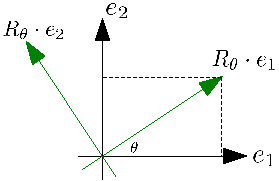
\includegraphics[scale=1.5]{figs/rotation-2D.pdf}
\end{center}
\begin{itemize}
\item Primeiro, o problema geom�trico � dotado de uma nota��o s�mb�lica
\item Seja o espa�o vetorial o plano 2D ($\mathbb R^2$)
\item A rota��o � uma transforma��o linear do plano no plano, indicada por $\text{Rot}$
\item Para chegarmos a n�meros (afinal, o curso � \emph{num�rico}), precisamos especificar coordenadas.  Seja o sistema de coordenadas indicado por uma base $E = \{e_1, e_2\}$ e
origem $O$. 
\item A rota��o ser� especificada por um �ngulo $\theta$ medido a partir de
  $e_1$, no sentido anti-hor�rio.
\item Para rotacionar o objeto (conjunto de pontos), precisamos saber como
  rotacionar um ponto. Em seguida, aplicamos o mesmo procedimento a todos os
  pontos. 
\item Pelo diagrama acima, a rota��o de um ponto em $e_1$ � $(\cos\theta, \sin\theta)^\top$, e
  de um ponto em $e_2$ � $(-\sin\theta,\cos\theta)^\top$.
\item Como vimos, basta colocar esses vetores na coluna da matriz de rota��o:
\[
  R_\theta = \mathcal M_E^E(\text{Rot}) = 
\begin{bmatrix} 
\cos\theta & -\sin\theta\\
\sin\theta &  \cos\theta
\end{bmatrix}
\]
\draftnote{Usar $R(\theta)$}
\item O sistema de
coordenadas n�o � rotacionado; apenas os pontos do plano s�o rotacionados,
fixando-se o sistema de coordenadas. 
\item Isso � modelado pela nota��o simb�lica como $\mathcal M_E^E(\text{Rot})$, onde a base � fixa, e a
  transforma��o � $\text{Rot}$.
\item Seguindo-se a nota��o e o racioc�nio de forma cuidadosa, a d�vida usual
  quanto ao sinal de $\sin\theta$ na matriz desaparece. Controle a ansiedade!
\item Outra vantagem � que o mesmo m�todo funciona para qualquer dimens�o (3D,
  4D, etc)
\end{itemize}

A seguinte ideia vale para montar a representa��o num�rica de uma matriz de
rota��o em qualquer dimens�o:
\begin{prop}
As \emph{colunas} duma matriz de rota��o s�o a rota��o dos vetores base
$e_1, \ldots, e_n$, escritas nesta pr�pria base.
As \emph{linhas} da matriz de rota��o s�o os vetores unit�rios que s�o levados
aos vetores base \emph{ap�s} a rota��o.
\end{prop}

\subsection{Rota��es 3D}

\begin{pbm}
  Rotacionar uma \emph{base} 3D em torno da origem, e escrever a matriz que
  realiza a mudan�a de base para um ponto arbitr�rio.
\end{pbm}

\begin{itemize}
\item A primeira dificuldade em definir os n�meros de matrizes de rota��o 3D �
  definir quais �ngulos geom�tricos s�o positivos (rota��es anti-hor�rias)
\end{itemize}

\begin{defi}(orienta��o) Uma base � dita \emph{de m�o-direita} quando as
  rota��es por �ngulos positivos s�o tais que, olhando-se de um vetor base em
  dire��o � origem, uma rota��o anti-hor�ria por $+90^o$ leva um eixo positivo em
  outro eixo positivo.
\end{defi}

\begin{itemize}
\item As regras da m�o direita vistas em cursos de f�sica permitem definir
  na pr�tica a orienta��o de uma base
\item O que nos interessa � a seguinte tabela:
\end{itemize}
\begin{center}
\begin{tabular}{c c} 
Se o eixo de rota��o � & A dire��o de rota��o por �ngulo positivo �\\
$x$	& $y \to z$ \\
$y$	& $z \to x$ \\
$z$	& $x \to y$ 
\end{tabular}
\end{center}

Como revis�o, a figura abaixo ilustra os graus de liberdade de uma rota��o e
seus nomes em ingl�s, no caso de um drone
\begin{center}
  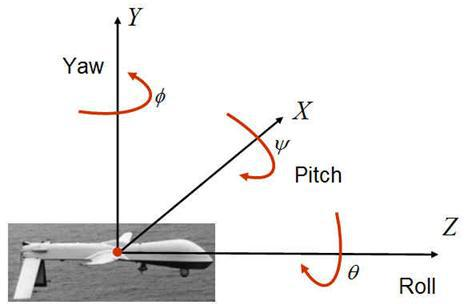
\includegraphics[scale=0.8]{figs/yaw-pitch-roll.jpg}
\end{center}
Em termos de tais �ngulos, a matriz de rota��o $R = \mathcal M^A_B(id)$ (neste
caso, de mudan�a de base, e n�o de uma rota��o geom�trica, pois os pontos s�o
fixos) pode ser decomposta como 
$R(\theta,\phi,\psi) =
R_z(\theta)R_y(\phi)R_x(\psi)$, onde
\begin{align}
R_z(\theta) &= \begin{bmatrix}
\cos\theta & \sin\theta & 0\\
-\sin\theta & \cos\theta & 0\\
0 & 0 & 1
\end{bmatrix}\\
%
R_y(\phi) &= \begin{bmatrix}
\cos\phi & 0 & -\sin\phi\\
0 & 1 & 0\\
\sin\phi &0 &\cos\phi
\end{bmatrix}\\
%
R_x(\psi) &= \begin{bmatrix}
1 & 0 & 0\\
0 & \cos\psi & \sin\psi\\
0 &-\sin\psi & \cos\psi
\end{bmatrix}
\end{align}
Note que cada coluna � obtida atrav�s da nossa nota��o:
\begin{equation}
  \mathcal X_B(v) = \mathcal M^A_B(id)\mathcal X_A(v),
\end{equation}
aplicada aos vetores base, onde a transforma��o linear $L$ aqui � $id$ pois
estamos fixando os pontos, mas estamos realizando uma mudan�a de base de $A$
para $B$. 
\begin{itemize}
\item A coluna i da matriz � ent�o $\mathcal X_B(a_i)$. Em outras palavras,
  nossa tarefa num�rica � escrever cada vetor base $a_i$ \emph{n�o-rotacionado} em termos
  dos vetores \emph{rotacionados}.
\end{itemize}
\begin{exer}
  Explique detalhadamente como obter a primeira coluna de $R_z(\theta)$.
\end{exer}

A forma final de $R(\theta,\phi,\psi) = R_z(\theta)R_y(\phi)R_x(\psi)$ para
uma rota��o arbitr�ria seria: 
\begin{align}
\begin{bmatrix}
\cos\theta\cos\phi & \cos\theta\sin\phi\sin\psi + \sin\theta\cos\psi & 
-\cos\theta\sin\phi\cos\psi + \sin\theta\sin\psi\\
%
-\sin\theta\cos\phi & -\sin\theta\sin\phi\sin\psi + \cos\theta\cos\psi &
\sin\theta\sin\phi\cos\psi + \cos\theta\sin\psi\\
%
\sin\phi & -\cos\phi\sin\psi & \cos\phi\cos\psi
\end{bmatrix}
\end{align}
\begin{exer}
Mostre que esta � a inversa da matriz que realiza a rota��o de pontos,
mantendo-se a base fixa.
\end{exer}

\mynewpage
\chapter{Modelando Transforma��es R�gidas Numericamente}
\section*{Objetivos}
\begin{itemize}
\item Representa��o vetorial e num�rica de transforma��es r�gidas, nosso primeiro exemplo
  de transforma��es n�o-lineares (transla��o al�m de rota��o)
\item Fornecer exemplos mais pr�ticos para as aulas anteriores
\item Qual o poder de modelagem da �lgebra matricial? Que tipos de problemas
  interessantes podemos tratar com essa �lgebra simples?
\end{itemize}

\section*{Vimos} -- revisar conceitos da aula passada
\begin{itemize}
\item Como modelar rota��es com matrizes
\end{itemize}

\mynewpage
\chapter{Coordenadas Homog�neas}
\section*{Objetivos}
\begin{itemize}
\item Qual o poder de modelagem da �lgebra matricial? Que tipos de problemas
  interessantes podemos tratar com essa �lgebra simples?
\item O que podemos fazer apenas com multiplica��o matriz-vetor? 
\item Proje��o perspectiva
\item Pr�-requisito para aulas de sistemas lineares homog�neos mais adiante no
  curso
\item Pr�-requisito para exemplo de c�meras, proje��o e computa��o gr�fica 
  mais adiante no curso
\end{itemize}

\section*{Vimos} -- revisar conceitos da aula passada
\begin{itemize}
\item Como modelar rota��es e transla��es numericamente com multiplica��o de matriz-vetor
  seguida de uma soma de vetor
\end{itemize}

\mynewpage
\chapter{Resolvendo sistemas lineares por SVD}
\epigraph{SVD is the answer.\\What is your problem?}{Joseph Mundy}


\section*{Objetivos}
\begin{itemize}
\item T�cnica gen�rica para resolver sistemas lineares
\item T�cnica mais �til em engenharia para sistemas sobredeterminados por
  m�nimos quadrados usando SVD
\item Solu��o aproximada de equa��es contradit�rias t�picas de medi��es com
  erro
\item T�cnica a ser vista n�o � a mais eficiente, mas � a mais usada antes de
  algoritmos mais espec�ficos
\item Foco ser� no procedimento geral, sendo a teoria aprofundada adiante
\end{itemize}

\section*{Vimos} -- revisar conceitos da aula passada
\begin{itemize}
\item Toda matriz $A = V \Lambda U^\top$ (SVD) (ver Aula~\ref{ch:intro})
\item Dado um algoritmo que realize esta decomposi��o na sua linguagem favorita,
  como resolver sistemas lineares?
\item N�o ser� necess�rio saber o algoritmo SVD em si, apenas entradas e sa�das.
\end{itemize}

\section*{Introdu��o}

\begin{itemize} \item 
Central em �lgebra linear num�rica � resolver sistemas da forma
\begin{equation}
  Ax = b.
\end{equation}
\item Em Scilab ou Matlab, por exemplo, pode-se usar a barra invertida para cegamente tentar
obter uma solu��o:
\begin{equation}
  x = A\ b,
\end{equation}
onde a nota��o com a barra invertida ``\'' sugere que $x$ � $b$ dividido por
$A$, de alguma forma. 
\item O Scilab nesse caso escolhe o melhor algoritmo, e em geral
  ser� o SVD, conforme veremos nesta se��o.
\end{itemize}

\begin{itemize}
\item Na pr�tica, a matriz $A$ e o vetor $b$ consitem de medi��es com erro, repetidas
in�meras vezes. 
\item Devido a esse erro, n�o h� um $x$ que exatamente satisfa�a $Ax = b$.
\item Nesse caso, queremos um $x$ que satifa�a $Ax = b$ aproximadamente. Ou
  seja:
  \begin{equation}
    Ax \approx b,
  \end{equation}
  onde ``$\approx$'' aqui significa aproximado.
\item A t�cnica a ser descrita nesta aula � uma maneira pr�tica de usar o SVD.
\item Muitas vezes, uma biblioteca em C ter� o algoritmo SVD, por�m pode n�o ter
  outras fun��es pr�ticas para solu��o de sistemas lineares.
\item Nesta aula, veremos uma t�cnica que transforma a equa��o acima numa
  equa��o homog�nea do tipo $Ax \approx 0$, e em seguida resolve um problema de
  otimiza��o com SVD.
\end{itemize}

\section*{Homogeneizando Sistemas Lineares}

\begin{itemize}
\item Dado um sistema $Ax = b$, podemos gerar um sistema equivalente $\tilde A \tilde
x = 0$. Dizemos que ``homogeneizamos o sistema''. 
\item O truque tem a ver com coordenadas homog�neas, mas o procedimento a seguir
  pode ser compreendido mesmo sem lembrar da Aula~\ref{ch:homogeneas}.
\item Suponha que a matriz $A$ seja $2\times 2$. O sistema $Ax = b$ ficaria:
\begin{equation}
\left\{
\begin{aligned}
  &a_{11}x_1 + a_{12}x_2 = b_1\\
  &a_{21}x_1 + a_{22}x_2 = b_2
\end{aligned}
\right.
\end{equation}
\item Note que apenas $b_1$ e $b_2$ n�o est�o acompanhados de vari�veis
\item Podemos fazer todos os termos conterem vari�veis (homog�neos)
  multiplicando-se todas as equa��es (em ambos os lados) por uma nova vari�vel
  $w$, sem alterar o resultado:
\begin{equation}
\left\{
\begin{aligned}
  &a_{11}x_1w + a_{12}x_2w = b_1w\\
  &a_{21}x_1w + a_{22}x_2w = b_2w
\end{aligned}
\right.
\end{equation}
Agora, podemos definir novas vari�veis $\tilde x_1 = x_1w$, $\tilde x_2 = x_2w$, de
forma que nosso novo vetor $\tilde x$ fique:
\begin{equation}
  \begin{bmatrix}
  \tilde x_1\\
  \tilde x_2\\
  \tilde x_3\\
  \end{bmatrix} \doteq 
  \begin{bmatrix}
  w x_1\\
  w x_2\\
  w
  \end{bmatrix} = w 
  \begin{bmatrix}
  x_1\\
  x_2\\
  1
\end{bmatrix}.
\end{equation}
Assim:
\begin{equation}
  \begin{bmatrix}
    a_{11} & a_{12} & -b_1\\
    a_{21} & a_{22} & -b_2
  \end{bmatrix}
  \begin{bmatrix}
  \tilde x_1\\
  \tilde x_2\\
  \tilde x_3\\
  \end{bmatrix}
  = 0
\end{equation}
\item Tal equa��o � homog�nea:
  \begin{equation}
    \tilde A\tilde x = 0
  \end{equation}
  A solu��o ser� o Kernel de $A$, $\ker A$ (n�cleo de A).
\item Logo, usando coordenadas homog�neas, podemos reduzir qualquer sistema
  linear n�o-homog�neo a um sistema linear homgo�neo
\item Torna-se central, ent�o, saber resolver:
  \begin{equation}
    Ax = 0, \ \ \ \ \text{ para } |x| \neq 0
  \end{equation}
\item Por exemplo, exigindo $|x| = 1$
\item Uma vez encontrado algum elemento $\tilde x$ do espa�o de solu�ao $\ker
  \tilde A$, para um sistema $\tilde A\tilde x =0$, podemos obter a solu��o para
  os sistema original $Ax=b$ 
\item Basta normalizar $\tilde x$ para obter $w = 1$ (sistema original), o que
  ocorre fazendo-se:
  \begin{equation}
  x = \begin{bmatrix}
  \tilde x_1 / \tilde x_3\\
  \tilde x_2 / \tilde x_3\\
  \end{bmatrix}
  \end{equation}
\end{itemize}

\section*{Solu��o aproximada por SVD: m�todo pr�tico}
Resolver o sistema aproximado
\begin{equation}
  Ax \approx 0, \ \ \ \ \text{ e } |x| = 1,
\end{equation}
� o mesmo que exigir que $Ax$ � pequeno. Ou seja, queremos resolver o seguinte
problema de otimiza��o
\begin{equation}
  \argmin_{|x|=1} |Ax|.
\end{equation}
\begin{itemize}
\item Se imaginarmos $x$ como um c�rculo ou esfera unit�ria, $|Ax|$ ser� m�nimo
  na dire��o do vetor singular correspondente ao menor valor singular, ou seja,
  basta calcular a SVD. (isto foi visto intuitivamente nas aulas anteriores)
\item Algebricamente, temos que, pelo SVD de $A$:
  \begin{equation}
    |Ax| = |V\Lambda U^\top x| = |\Lambda U^\top x|,
  \end{equation}
  onde a �ltima passagem se deve ao fato de $V$ ser ortogonal, ou seja, n�o
  altera a norma.
\item Logo, queremos minimizar
  \begin{equation}
    |\Lambda U^\top x| \ \ \ \text{ tal que } |x| = 1
  \end{equation}
\item Como $|x| = |U^\top x|$, podemos definir $y \doteq U^\top x$. 
\item Ent�o, queremos minimizar
  \begin{equation}
    |\Lambda y| \ \ \ \text{ tal que } |y| = 1.
  \end{equation}
\item Como $\Lambda$ � diagonal, e os algoritmos retornam os valores singulares
  $\sigma_i$ na ordem decrescente, ent�o a solu��o � 
  \begin{equation}
    y = \begin{bmatrix}0 \\ 0 \\ \vdots\\ 1\end{bmatrix}
  \end{equation}
  
\end{itemize}

\mynewpage
\chapter{Aprofundando em SVD}

\section*{Objetivos}
\begin{itemize}
\item Defini��o formal de SVD ap�s ter visto como usar
\item Demonstra��o do SVD --  um dos teoremas mais importantes da �lgebra linear
  moderna, por causa de um algoritmo de �lgebra lihnear num�rica.
\item Conex�o com autovalores e autovetores
\item Gancho para an�lise de algoritmos para SVD e para autovalores e
  autovetores do Golub (este curso � estilo \emph{top-bottom})
\item Interpreta��es gr�ficas de autovalores, autovetores, valores singulares e
  vetores singulares
\end{itemize}

\section*{Vimos} -- revisar conceitos da aula passada
\begin{itemize}
\item J� vimos SVD operacionalmente: $A = U\Lambda V^\top$
\item J� vimos como SVD pode ser usado para resolver sistemas $Ax \approx b$ de
  forma pr�tica, mesmo n�o sendo a mais eficiente em todos os casos.
\item Veremos agora a defini��o formal de SVD
\end{itemize}

\begin{itemize}
\item Um autovetor de trasnforma��o linear � um vetor cuja dire��o � preservada pela
 transforma��o linear:
\begin{center}
  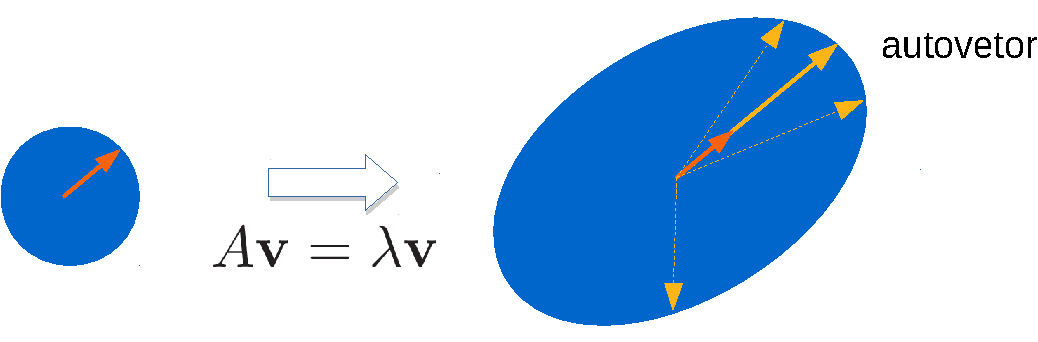
\includegraphics[scale=0.9]{figs/eigenvector.pdf}
\end{center}
\item A figura acima mostra que a matriz $A$ estica o disco a uma elipse, 
  uma manifesta��o num�rica de uma transforma��o linear
\item Se imaginarmos que o disco � feito de borracha, e a matriz $A$ � tal que 
  o esticamento � feito puxando-se os pontos do disco original ao longo de 
  eixos da elipse, ent�o a dire��o dos pontos ao longo dos eixos n�o se altera,
  pois os pontos apenas movem ao longo dos eixos durante o esticamento
\item Para tais tipos de matrizes, podemos tomar todos os eixos da elipse como
  uma base:
\begin{center}
  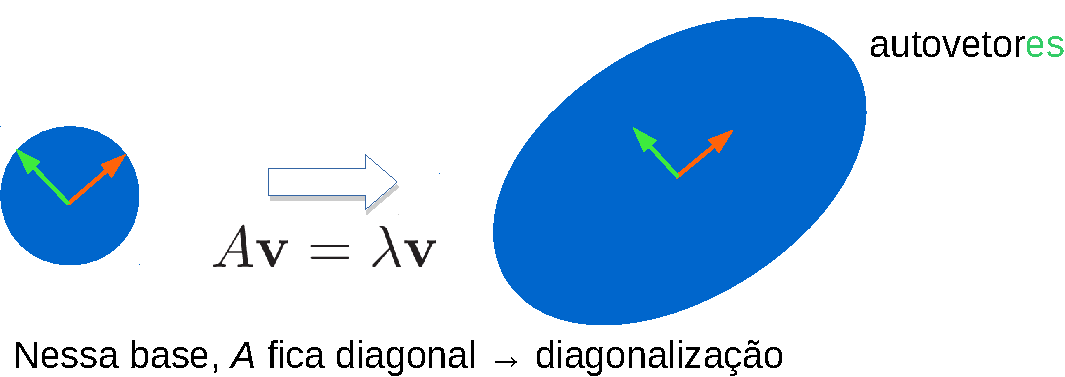
\includegraphics[scale=0.9]{figs/all-eigenvectors.pdf}
\end{center}
\item Como fica esse racioc�nio para \emph{qualquer} matriz $K$ de tamanho $m\times
  n$?
\item A resposta � SVD. Veja um esquema do enunciado que veremos formalmente a
  seguir.
\begin{center}
  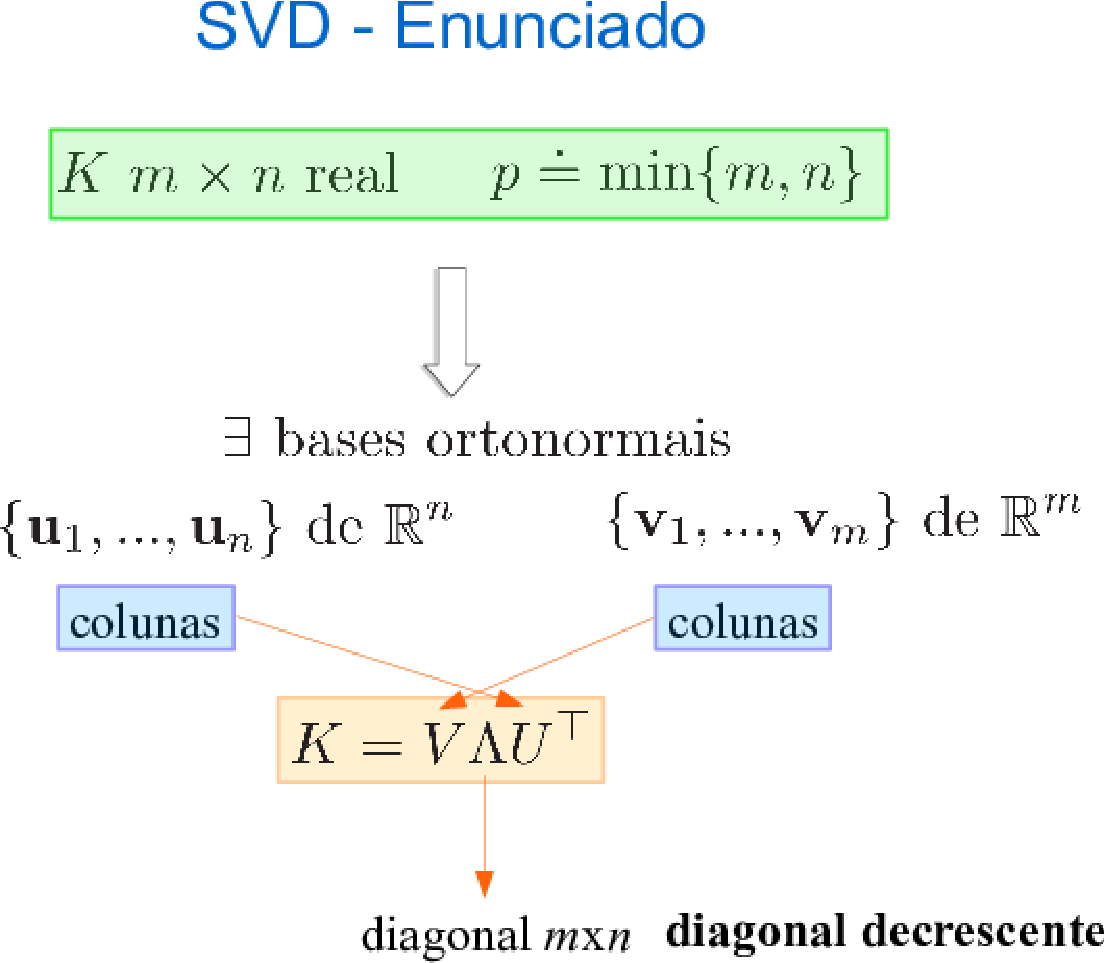
\includegraphics[scale=0.6]{figs/svd-enunciado.pdf}
\end{center}
\item Note que, diferenciar de $A$ acima, apropriada para autovetores e autovalores,
  iremos utilizar a letra $K$ para uma matriz geral.
\end{itemize}

\begin{teo} \emph{(Decomposi��o em Valores Singulares)}
  Seja $K$ uma matriz real $m\times n$ e $p \doteq \min \{m,n\}$
Ent�o existem bases ortonormais $\{u_1,\dots,u_n\}$ de $\mathbb{R}^n$
e $\{v_1,\dots,v_m\}$ de $\mathbb R^m$ tais que
\begin{equation}
  K = V \Lambda U^\top,
\end{equation}
com $\Lambda$ matriz diagonal $m\times n$ com elementos diagonais
\begin{equation}
  \Lambda = 
  \begin{bmatrix}
    \sigma_1 & 0 & \dots & 0\\
    0 & \sigma_2 & \ddots & \vdots \\
    \vdots & \ddots & \ddots & 0 \\
    0 & \dots & 0 & \sigma_{\boldsymbol{n}}\\
    0 & \multicolumn{2}{c}{\dots} & 0\\
    \vdots & & & \vdots\\
    0 & \multicolumn{2}{c}{\dots} & 0
  \end{bmatrix}
\end{equation},
se $m > n = p$, ou 
\begin{equation}
  \Lambda = 
  \begin{bmatrix}
    \sigma_1 & 0 & \dots & 0 &0 & \multicolumn{2}{c}{\dots} & 0\\
    0 & \sigma_2 & \ddots & \vdots & \vdots & & & \vdots\\
    \vdots & \ddots & \ddots & 0 & \vdots & & & \vdots\\
    0 & \dots & 0 & \sigma_{\boldsymbol{m}}& 0 & \multicolumn{2}{c}{\dots} & 0
  \end{bmatrix}
\end{equation}, se $p = m < n$,
e as matrizes 
$$
V =
\begin{bmatrix}
  | &  &  |\\
  v_1 & \dots & v_m\\
  | &  &  |
\end{bmatrix}_{m\times m}
\text{ \ \ \ e \ \ } 
U =
\begin{bmatrix}
  | &  &  |\\
  u_1 & \dots & u_n\\
  | &  &  |
\end{bmatrix}_{n\times n}
$$
s�o ambas ortogonais. Os n�meros $\sigma_1,\dots,\sigma_p$ s�o chamados valores
singulares de $K$.
\end{teo}
\begin{proof}
  \begin{itemize}
  \item 
  Note que $K$ define uma transforma��o linear $\mathbb R^n \to \mathbb R^m$.
  \item Note-se, tamb�m, que $K$ � arbitr�ria. A id�ia do teorema � montar uma matriz
    sim�trica, adequada para o c�lculo de autovalores e autovetores. Dessa
    forma, o SVD � reduzido a autovalroes e autovetores.
  \item H� duas formas �bvias de montar uma matriz sim�trica a partir de $K$: 
  \item A primeira forma � $K = K^\top K$, uma matriz sim�trica de tamanho $n\times n$.
  \item A segunda � $K = KK^\top$, uma matriz sim�trica de tamanho $m\times m$.
  \item Os autovetores dessas matrizes d�o os vetores singulares
  \item Os autovalores dessas matrizes s�o iguais e d�o os valores singulares ao
    quadrado
  \item A seguir, vamos detalhar esses passos de uma forma menos redundante
  \end{itemize}
  
  \paragraph{1. Monta-se uma base ortonormal para $\mathbb R^n$ (dom�nio)}
  \begin{itemize}
  \item Seja $A = K^\top K$, a qual � real e sim�trica, satisfazendo as hip�teses do
  teorema espectral
\item Sejam $u_1,\dots,u_n$ os vetores da base ortonormal de $\mathbb R^n$ que
  diagonaliza $A$
\item Sejam $\lambda_1\geq \dots \geq \lambda_n$ tal que
  \begin{equation}
    Au_i = \lambda u_i, \ \ \ i=1,\dots,n.
  \end{equation}
  \end{itemize}
  
  \paragraph{2. Monta-se uma base ortonormal para $\mathbb R^m$ (contra-dom�nio)}
  Seja $n_0$ o �ndice do menor $\lambda_i$ e 
  \begin{equation}
    w_i \doteq K u_i, \ \ \ i = 1,\dots,n_0 \leq p.
  \end{equation}
  Ent�o os $w_i$ s�o ortogonais:
  \begin{equation}
    w_i^\top w_j = u_i^\top K^\top K u_j = u_i^\top A u_j = \lambda_j u_i^\top
    u_j = \lambda_j \delta_{ij},
  \end{equation}
  onde $\delta_{ij}$ � o delta de Kronecker ($1$, se $i=j$, $0$ se $i\neq j$)
  para $i,j = 1,\dots,n_0$

Definem-se 
\begin{align}
  v_i &\doteq \frac{w_i}{|w_i|} = \frac{K u_i}{|K u_i|}, \ \ \ i=1,\dots,n_0,\\
  \sigma_i &\doteq |Ku_i|.
\end{align}

Logo, $v_1,\dots,v_{n_0}$ s�o ortonormais e 
\begin{align}
  Ku_i = \sigma_i v_i
\end{align}
e
\begin{equation}
  K^\top v_i = \frac{K^\top K}{\sigma_i}u_i = \frac{\lambda_i}{\sigma_i}u_i.
\end{equation}
Ademais, $\lambda_i = \sigma_i^2$, $i = 1,\dots,n_0$, pois
\begin{align}
  \lambda_1 &= \lambda_i u_i^\top u_i = (\lambda_i u_i)^\top u_i = (Au_i)^\top
  u_i \\
  &= (K^\top K u_i)^\top u_i = u_i^\top K^\top K u_i = (K u_i)^\top (K u_i)\\
  &= \sigma_i^2V_i^\top V_i = \sigma^2_i, \ \ \ i=1,\dots,n_0
\end{align}

\begin{itemize}
\item Definimos $\sigma_i \doteq 0$, para $n_0 < i \leq p$, se existir tal $i$
\item Sejam $v_i$, $n_0 < i \leq m$, vetores ortonormais completando
$v_1,\dots,v_{n_0}$ a uma base ortonormal de $\mathbb R^m$
\item Montando-se as matrizes 
$$
V =
\begin{bmatrix}
  | &  &  |\\
  v_1 & \dots & v_m\\
  | &  &  |
\end{bmatrix}_{m\times m}
\text{ \ \ \ e \ \ } 
U =
\begin{bmatrix}
  | &  &  |\\
  u_1 & \dots & u_n\\
  | &  &  |
\end{bmatrix}_{n\times n},
$$
as propriedades enunciadas s�o satisfeitas.
\end{itemize}
\end{proof}

\paragraph{Discuss�o 1}

\begin{itemize}
\item Dada a decomposi��o SVD $K = V \Lambda U^\top$,
  multiplicando-se ambos os lados por $U$, tem-se:
  \begin{equation}
    K U = V \Lambda,
  \end{equation}
  ou seja 
  \begin{equation}
    K u_i = \sigma_i v_i,
  \end{equation}
  uma equa��o an�loga � defini��o de autovalores e autovetores.
\item Na equa��o, parece ser arbitr�rio que ao se multiplicar um vetor, obt�m-se
  o m�ltiplo de outro vetor
\item � importante que $u_i$'s e $v_i$'s definem bases ortogonais para $\mathbb
  R^n$ e $\mathbb R^m$, respectivamente
\end{itemize}

\paragraph{Discuss�o 2}
\begin{itemize}
\item Se $K = V \Lambda U^\top$, ent�o $K^\top K = U\Lambda V^\top V \Lambda
  U^\top = U \Lambda^2 U^\top$, uma diagonaliza��o comum com autovetores e
  autovalores
\item E $K K^\top = V \Lambda ^2 V^\top$, uma diagonaliza��o comum com autovetores e
\item O SVD fornece bases ortonormais aos seguintes espa�os fundamentais de $K$:
\begin{empheq}[left=\empheqlbrace]{align}
  v_1,\dots, v_r & \text{ base ortonormal de } \img(K)\\
  v_{r+1},\dots, v_m & \text{ base ortonormal de } \ker(K^\top)\\
  u_{1},\dots, u_r & \text{ base ortonormal de } \img(K^\top)\\
  u_{r+1},\dots, u_n & \text{ base ortonormal de } \ker(K)
\end{empheq}
  
\end{itemize}

\mynewpage
\chapter{Decomposi��o QR}

\section*{Objetivos}
\begin{itemize}
\item Principais algoritmos de decomposi��o QR
\end{itemize}

\section*{Vimos} -- revisar conceitos da aula passada
\begin{itemize}
\item Vimos a decomposi��o SVD. 
\item A decomposi��o QR � um passo importante em muitos outros algoritmos,
  al�m de ser melhor em casos espec�ficos
\end{itemize}


\section{Revis�o de matrizes ortogonais}\label{sec:ortogonais:rev}

\begin{itemize}
\item Uma matriz quadrada $U$ � ortogonal se $U^\top U = U U^\top = I$
\item Propriedade: $\det U = \pm 1$
\item Matrizes de rota��o s�o matrizes ortogonais com determinante $+1$
\item Matrizes ortogonais preservam produto interno e norma: $(Ux)^\top Ux = x^\top U^\top U x =
  x^\top x$
\end{itemize}

\section{Decomposi��o QR por matrizes Givens}

\begin{defi}
  A decomposi��o QR de uma matriz $A$ � da forma:
  \begin{center}
  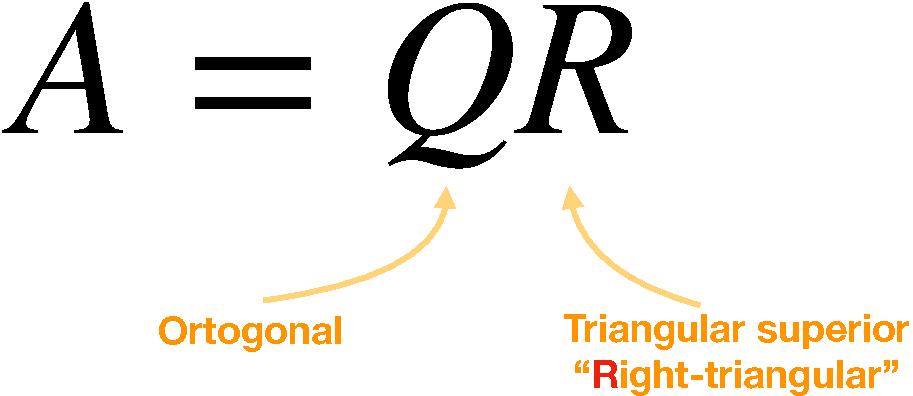
\includegraphics[scale=0.6]{figs/qr.pdf}
  \end{center}
\end{defi}
\begin{itemize}
\item Existem tamb�m decomposi��es similares � QR, todas chamadas ``QR'' em um sentido
amplo: QL, LQ, RQ, onde ``L'' � triangular inferior (de ``left /
lower-triangular'').
\item Antes de entrar em detalhes t�tnicos, vejamos um algoritmo simples para matrizes $3\times
  3$ usando matrizes especiais chamadas ``Givens''
\end{itemize}

\begin{defi}
  Uma matriz Givens de rota��o � uma rota��o em torno de um dos eixos $x, y$ ou
  $z$:
  \begin{equation}
    Q_x =
    \begin{bmatrix}
      1 & 0 & 0\\
      0 & c & -s\\
      0 & s & c
    \end{bmatrix},\ \ 
    Q_y =
    \begin{bmatrix}
      c & 0 & s\\
      0 & 1 & 0\\
      -s & 0 & c
    \end{bmatrix},\ \ 
    Q_z =
    \begin{bmatrix}
      c & -s & 0\\
      s & c & 0\\
      0 & 0 & 1
    \end{bmatrix}
  \end{equation},
  onde $c = \cos \theta$ e $s = sen \theta$.
\end{defi}

\begin{itemize}
\item 
Ao fazer a opera��o $A\cdot Q_z$ para uma matriz $A$, sua �ltima coluna n�o
muda, e as duas primeiras � combina��o linear das duas primeiras de $A$.
\item (multiplicar $AQ_z$ explicitamente para constatar isso)
\item Podemos escolher $\theta$ de forma a zerar qualquer entrada desejada das
primeiras colunas
\item Por exemplo, para setar o elemento (2,1) do resultado para zero,
  \begin{equation}
    \begin{bmatrix}
      a_{11} & a_{12} & a_{13}\\
      a_{21} & a_{22} & a_{23}\\
      a_{31} & a_{32} & a_{33}
    \end{bmatrix}
    \begin{bmatrix}
      c & -s & 0\\
      s & c & 0\\
      0 & 0 & 1
    \end{bmatrix}
    =
    \begin{bmatrix}
      c a_{11} + s a_{12} & -s a_{11} +c a_{12} & a_{13}\\
      c a_{21} + s a_{22} & -s a_{21} +c a_{22} & a_{23}\\
      c a_{31} + s a_{32} & -s a_{31} +c a_{32} & a_{33}\\
    \end{bmatrix}.
  \end{equation}
  Impondo
\begin{empheq}[left=\empheqlbrace]{align}
  &c a_{21} + s a_{22} = 0\\
  &c^2 + s^2 = 1,
\end{empheq}
encontramos $c$ e $s$.
\end{itemize}

\subsection{Estrat�gia de Algoritmo RQ por matrizes Givens}
\begin{itemize}
\item Iremos descrever uma estrat�gia para o algoritmo RQ, sendo o QR an�logo.
\item Zerar a parte inferior da matriz, uma entrada por vez, multiplicando-se
  por matrizes Givens, cuidando-se para n�o modificar as entradas que j� foram
  anuladas
\end{itemize}

\begin{algorithm}
  \caption{Decomposi��o RQ por matrizes Givens}
  \textbf{Entrada:} matriz $3\times 3$ A
  
  \textbf{Sa�da:} $R$ e $Q$ tal que $A = RQ$\\
  \ \\
  \emph{in�cio}
  \begin{enumerate}
  \item Multiplica-se por $Q_x$ tal que $A_{32} \to 0$ 
  \item Multiplica-se por $Q_y$ tal que $A_{31} \to 0$ (isso n�o muda
      $A_{32}$ pois n�o afeta a coluna 2
    \item Multiplica-se por $Q_z$ tal que $A_{21} \to 0$ ($A_{31}$ e $A_{32}$
      permanecem zeradas, j� que as primeiras colunas s�o substitu�das por
    combina��es lineares delas mesmas)
  \item Observa��o: outras sequ�ncias de rota��es Givens podem tamb�m resultar na
  mesma coisa
  \item $AQ_x Q_y Q_z = R \implies A = R Q^\top_z Q^\top_y Q^\top_x = RQ$
  \end{enumerate}
  \emph{fim}
\end{algorithm}


\mynewpage
\chapter{Matrizes Householder para Decomposi��o QR}

\section*{Objetivos}
\begin{itemize}
\item Ilustar o importante assunto de Matrizes Householder em �lgebra linear
  num�rica
\end{itemize}

\section*{Vimos} -- revisar conceitos da aula passada
\begin{itemize}
\item Vimos a decomposi��o QR por matrizes Givens. 
\item Para matrizes grandes $n \times n$, com $n \gg 3$, � melhor usar matrizes
  de Householder, que s�o da forma:
  \begin{equation}
    H_v = I - 2 \frac{vv^\top}{v^\top v}
  \end{equation}
\item Note que � ortogonal e sim�trica (mostrar em aula)
\end{itemize}

\begin{prop}
  Seja 
  \begin{equation}
    v = x \pm |x|e_1,
  \end{equation}
  onde $e_1$ � um vetor base. Ent�o
  \begin{equation}
    H_v x = \mp |x|e_1.
  \end{equation}
  Ou seja, $H_v$ � uma matriz ortogonal que leva $x$ a um m�ltiplo de $e_1$,
  portanto zerando todas as outras entradas / coordenadas.
\end{prop}

\begin{proof}
  \begin{equation}
  H_vx = I - 2 \frac{(x \pm |x|e_1)(x \pm |x| e_1)^\top x}{(x \pm |x|e_1)^\top(x \pm |x| e_1)}
  \end{equation}
  \begin{itemize}
  \item Exerc�cio em aula: terminar esta prova
  \end{itemize}
\end{proof}

Toma-se 
\begin{equation}
v = x + sign(x_1) |x| e_1
\end{equation}
\begin{center}
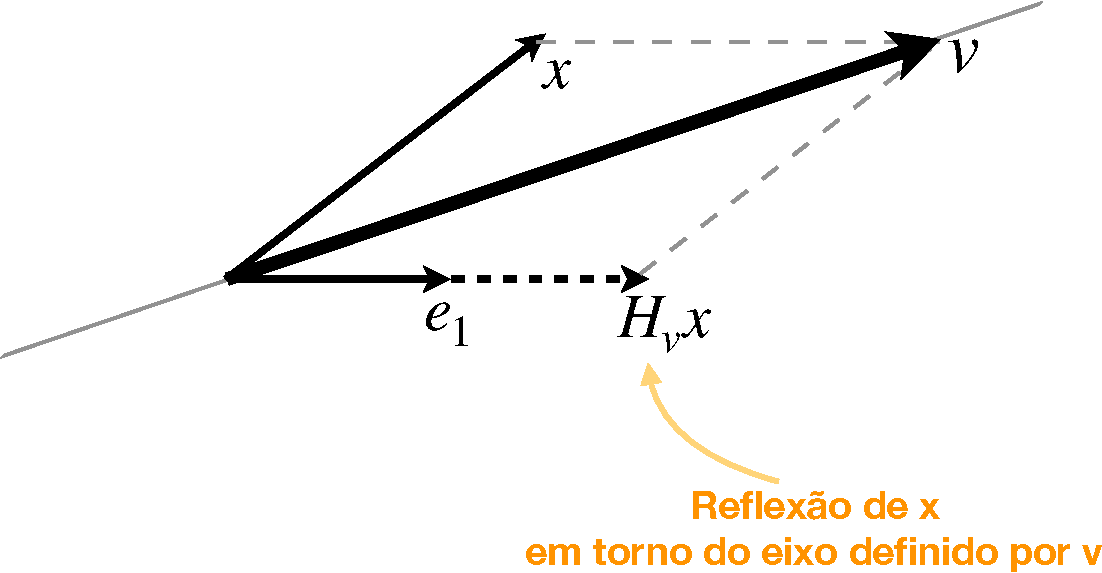
\includegraphics[scale=0.6]{figs/householder.pdf}
\end{center}

Para uma dada matriz $A$, tomando-se $x$ sua primeira coluna e $v$ como acima,
ent�o $H_v A$ vai zerar quase toda primeira coluna, que fica
\begin{equation}
  \begin{bmatrix}
    |x|\\
    \vdots\\
    0
  \end{bmatrix}.
\end{equation}

Continuando a multiplica��o � esquerda por rota��es Householder adequadas,
podemos triangular a matriz:
\begin{align}
  \tilde Q A &= R\\
  A &= \tilde Q^\top R = QR
\end{align}
que � a decomposi��o QR de $A$.

Tais matrizes Householder adequadas s�o da seguinte forma:

\mynewpage
\chapter{Decomposi��o de Cholesky}

\section*{Objetivos}
\begin{itemize}
\item Compreender aspectos b�sicos da decomposi��o de cholesky
\end{itemize}

\section*{Vimos} -- revisar conceitos da aula passada
\begin{itemize}
\item Vimos as decomposi��es QR e SVD. 
\item Na demonstra��o do SVD, tinhamos matrizes sim�tricas A montadas a partir
  de $K$: $A = K^\top K$ ou $A = KK^\top$
\item Em algumas aplica��es, temos o contr�rio: dada uma matriz sim�trica $A$, como
  encontrar $K$ tal que $A = K^\top K$ ou $A = K K^\top$
\end{itemize}

\begin{itemize}
\item A decomposi��o de Cholesky � um tipo de ra�z quadrada de matrizes 
\item � uma ra�z quadrada �til quando a matriz � sim�trica, positiva definida
  (revisaremos a defini��o)
  \begin{itemize}
  \item Muitos casos pr�ticos s�o desse tipo
  \item Nesses casos, Cholesky � bem mais r�pido e est�vel que alternativas
  \end{itemize}
\item Esta decomposi��o � parte do ferramental fundamental de �lgebra linear
  num�rica
\item Dada uma matriz $A$, a decomposi��o de cholesky retorna $K$ tal que $A =
  KK^\top$, se poss�vel
\item Se $A$ fosse um n�mero, seria exigido que $A$ fosse positivo (e real),
  caso quisessemos uma ra�z quadrada $K$ real
\item Similarmente, para uma matriz $A$ quadrada $n \times n$, exigimos que
  seja:
  
  \begin{tabular}{c | c}
    \textbf{Condi��o na matriz} & \textbf{Condi��o correspondente nos
    autovalores}\\\hline\hline
  Sim�trica & autovalores reais\\
  Positiva-definida & autovalores positivos
  \end{tabular}
\end{itemize}

\begin{defi}
  $A$ � sim�trica positiva-definida se todos seus autovalores s�o positivos
\end{defi}

\begin{teo} Os seguintes fatos s�o verdadeiros:
  \begin{enumerate}
  \item Uma matriz sim�trica $A$ � positiva-definida $\iff x^\top A x > 0,
    \forall x \neq 0$
  \item Uma matriz $A$ � sim�trica positiva definida $\implies$ existe uma �nica
    matriz $K$ triangular superior e real com diagonal positiva tal que $A =
    KK^\top$
  \end{enumerate}
\end{teo}

\begin{proof}\ \\
  
  \begin{enumerate}
  \item 
    \begin{enumerate}
    \item Por decomposi��o em autovalores e autovetores, temos $A = U D U^\top$
    \item Ida: 
      \begin{equation}
        x^\top U D U^\top x = y D y^\top = \sum d_{ii}y_i^2 > 0, \forall x
      \end{equation}
    \item Volta:
      \begin{equation}
        x^\top A x > 0 \implies x^\top U D U^\top x > 0 \implies y^\top D y > 0,
        \forall y \text { onde } y = x^\top U.
      \end{equation}
      Colocando $y = e_i$, temos $d_{ii} > 0$
    \end{enumerate}
  \item 
    
    \begin{itemize}
    \item $A = U D U^\top$, com $D$ real positiva, ent�o tomemos a ``raiz quadrada
    de D'', 
    \begin{equation}
      D = E E^\top, \ \ \ \text{com } E \text{ diagonal.}
    \end{equation}
    \item Logo, $A = VV^\top$, onde $V = UE$. 
    \item A matriz $V$ n�o � necessariamente triangular superior. 
    \item Aplica-se, ent�o, a decomposi��o RQ da forma
      \begin{equation}
        V = KQ,
      \end{equation}
      o que d� 
      \begin{equation}
        A  = VV^\top = KQQ^\top K^\top = K K^\top
      \end{equation}
    \item Se as diagonais n�o forem positivas, basta multiplicar $K$ � direita
      por uma matriz com $\pm 1$'s nas diagonais -- isso n�o afetar� o produto
      $K^\top K$
    \item $K$ � �nica pois:
    \item Sejam $K_1$, $K_2$ com $K_1K_1^\top = K_2K_2^\top$. Ent�o 
      \begin{equation}
        K_2^{-1}K = K_2^\top K_1^{-\top} = D,
      \end{equation}
      duas matrizes tiangualres superiores e inferiores, respectivamente.
    \item Ademais, $K_2^{-1}K_1$ � igual a $(K_2^\top K_1^{-\top})^{-\top}$
    \item Logo, $D = D^{-\top}$ sendo, portanto, com entradas $\pm 1$. Como $K_1$
      e $K_2$ t�m diagonal positiva, este sinal � positivo.
    \end{itemize}
  \end{enumerate}
\end{proof}

Vejamos um primeiro algoritmo para decomposi��o de Cholesky de matrizes $3\times
3$:

\begin{algorithm}
  \caption{Algoritmo de Cholesky-Banachiewicz}
  \textbf{Entrada:} matriz $3\times 3$ A
  
  \textbf{Sa�da:} matriz $3\times 3$ $K$ tal que $A = KK^\top$\\
  \ \\
  \emph{in�cio}
  \begin{enumerate}
  \item Suponha $K$ triangular inferior $L$ e multiplique as matrizes:
  \begin{align}
    A &= LL^\top =
    \begin{bmatrix}
      L_{11} & 0 & 0\\
      L_{21} & L_{22} & 0\\
      L_{31} & L_{32} & L_{33}
    \end{bmatrix}
    \begin{bmatrix}
      L_{11} & L_{21} & L_{31}\\
      0 & L_{22} & L_{32}\\
      0 & 0 & L_{33}
    \end{bmatrix} = \\
    &= \begin{bmatrix}
      L_{11}^2 & \bullet & \bullet\\
      L_{21}L_{11} & L_{21}^2 + L_{22}^2 & \bullet\\
      L_{31}L_{11} & L_{31}L_{21} + L_{32}L_{22} & L_{31}^2 + L_{31}^2 +
      L_{33}^2 & L_{33}
    \end{bmatrix}.
  \end{align}
  Onde os s�mbolos ``$\bullet$'' denotam entradas sim�tricas.
\item Resolve-se os $L_{ij}$'s em termos de $A_{ij}$ linha por linha, iniciando
  pelo canto superior esquerdo:
  \begin{align}
    L_{jj} &= \sqrt{A_{jj} - \sum_{k=1}^{j-1} L_{jk}^2} > 0, \ \ \text{se $A$ �
    positiva definida}\\
    L_{ij} &= \frac{1}{L_{jj}} \left( A_{ij} - \sum_{k=1}{j-1} L_{ik}L_{jk}
    \right),\ \ \  \text{ para $i > j$}
  \end{align}
  \end{enumerate}
  \emph{fim}
\end{algorithm}

\mynewpage
\chapter{Revis�o de Scilab/Matlab/Python}

\section*{Objetivos}
\begin{itemize}
\item Introduzir resumo de aspectos matriciais de linguagem de programa��o
  \emph{script}, visando realiza�ao das tarefas
\item Geralmente dada no in�cio do curso. Fica a crit�rio do instrutor quando
  dar esta aula.
\end{itemize}

\mynewpage
\chapter{Exponenciais de Matrizes}


\section*{Objetivos}
\begin{itemize}
\item M�todos num�ricos para solu��o de equa��es n�o-lineares exigem a solu��o
  de uma fam�lia de sistemas lineares
\item Faz-se necess�rio obter essa fam�lia a partir de parametriza��es simples
\item S�ries de pot�ncia permitem gerar fam�lias de sistemas lineares expandindo
  a partir de matrizes simples.
\item A expans�o em s�rie pode ser uma base para algoritmos eficientes, mesmo n�o
  sendo em si um procedimento final
\item Base para aplica��es em sistemas din�micos e solu��o de equa��es n�o-lineares usando
  tera��o com sistemas lineares (m�todos de Newton, Gauss-Newton e afins).
\end{itemize}

\section*{Vimos} -- revisar conceitos da aula passada

\section{Matrizes Anti-Sim�tricas}

\begin{itemize}
\item Ser� �til revisarmos matrizes anti-sim�tricas e aprofundar neste assunto
\item Na Se��o~\ref{sec:ortogonais:rev}, revisamos matrizes ortogonais que ser�o
  �teis como exemplos nesta se��o.
\item Resta-nos revisar matrizes anti-sim�tricas
\item Matrizes anti-sim�tricas e ortogonais ser�o conectadas com 
exponenciais de matrizes
\item M�todos num�ricos relacionados ser�o obtidos e analisados, permitindo o
  uso de matrizes simples para expressar e parametrizar matrizes mais complicadas.
\end{itemize}

\begin{itemize}
\item Dado um vetor ${\bf v}=(v_1,v_2,v_3)^\top$, � poss�vel construir uma matriz anti-sim�trica com as componentes de ${\bf v}$ na forma
\begin{equation*}
[{\bf v}]_\times=
\begin{bmatrix}
0&-v_3&v_2\\
v_3&0&-v_1\\
-v_2&v_1&0
\end{bmatrix}.
\end{equation*}
\item A nota��o $[{\bf v}]_\times$, tamb�m denotada $\skewm{\vec v}$, indica
uma rela��o do produto desta matriz por um vetor qualquer $\vec u$ com o produto
vetorial entre $\vec u$ e ${\bf v}$. De fato, pode-se expressar o produto
vetorial por $\vec v$ atrav�s de multiplica��o de matriz:
\begin{equation*}
{\bf v} \times {\bf u} = [{\bf v}]_\times {\bf u} = ({\bf v}^\top [{\bf u}]_\times)^\top
\end{equation*}
\item Tal representa��o matricial de um produto vetorial tem grandes
  implica��es pr�ticas para o uso de t�cnicas matriciais na solu��o de equa��es
  envolvendo 3 dimens�es (mec�nica/cinem�tica).
\item Sabemos que o produto vetorial entre um vetor e ele mesmo � sempre o vetor nulo, portanto o vetor ${\bf v}$ � o vetor nulo � direita e � esquerda de $[{\bf v}]_\times$. Desta forma, esta matriz anti-sim�trica ser� sempre definida por seu vetor nulo.  
\end{itemize}

Observe, ainda, que uma matriz anti-sim�trica qualquer $M$ satisfaz a rela��o ${\bf v}^\top M\,{\bf v}=0.$ Pois,
\begin{equation*}
\begin{array}{rcl}
{\bf v}^\top M\,{\bf v}
&=&
\begin{pmatrix}
v_1&v_2&v_3
\end{pmatrix}
\begin{bmatrix}
0&m_{12}&m_{13}\\
-m_{12}&0&m_{23}\\
-m_{13}&-m_{23}&0
\end{bmatrix}
\begin{pmatrix}
v_1\\
v_2\\
v_3
\end{pmatrix}\\
&=&
\begin{pmatrix}
-v_2 m_{12}-v_3 m_{13}&v_1 m_{12}-v_3 m_{23}&v_1 m_{13}+v_2 m_{23}
\end{pmatrix}
\begin{pmatrix}
v_1\\
v_2\\
v_3
\end{pmatrix}\\
&=&
-v_1 v_2 m_{12}-v_1 v_3 m_{13}+v_1 v_2 m_{12}-v_2 v_3 m_{23}+v_1 v_3 m_{13}+v_2 v_3 m_{23}\\
&=&0.
\end{array}
\end{equation*}


\mynewpage
\chapter{Condicionamento de Sistemas Lineares}

(rascunho)


\section*{Objetivos}
\begin{itemize}
\item Definir n�mero de condicionamento $\kappa$ no caso de sistemas lineares
\item Dar uma ideia do que seria para sistemas n�o-lineares ou, mais
  especificamente, polinomiais, j� que o caso linear � usado a cada passo
\item Escalas e normaliza��es em sistemas lineares (ver HZ)
\item Que transforma��es iniciais podem tornar um algoritmo mais r�pido? mais
  est�vel?
\end{itemize}


\mynewpage
\chapter{To Do}
\begin{enumerate}
\item Explicar melhor como retas e planos sao nao-lineares
\item Figura de transforma��es nao-lineares e nao-diferenciaveis (rasgar, formar
  bicos, etc)
\item enviar para daiara, carlos, francisco
\item Aula: Transformacoes rigidas: Rotacao e translacao
\item Aula: Coordenadas homogeneas
\item Aula: QR householder, QR givens
\item Aula: Cholesky
\item Aula: SVD: teorema e demonstracao, algumas figs, relembrar autovalores
\item Aula: homogeneizacao de sistemas e uso de SVD sobredeterminado
\item Aula: Aplicacao em imagens
\item Aula: Aplicacao em cameras
\item Aula: Aplicacao em reconhecimento
\end{enumerate}

\mynewpage
\bibliographystyle{plainnat}
%\bibliographystyle{authordate}
\bibliography{shading,multiview,motion,Kimia,bib-header,video,math-books,math,psych-books,metric,edge,leymarie_pami_scaffold,vision-books,vision,recognition,optical-flow,indexing,proceedings}


\end{document}
